% Options for packages loaded elsewhere
\PassOptionsToPackage{unicode}{hyperref}
\PassOptionsToPackage{hyphens}{url}
%
\documentclass[
  ignorenonframetext,
]{beamer}
\title{Spatial modeling with \texttt{INLA} and \texttt{inlabru}}
\subtitle{University of Zurich, March, 2022}
\author{Instructor: Sara Martino}
\date{}
\institute{Department of Mathematical Science (NTNU)}

\usepackage{pgfpages}
\setbeamertemplate{caption}[numbered]
\setbeamertemplate{caption label separator}{: }
\setbeamercolor{caption name}{fg=normal text.fg}
\beamertemplatenavigationsymbolsempty
% Prevent slide breaks in the middle of a paragraph
\widowpenalties 1 10000
\raggedbottom
\setbeamertemplate{part page}{
  \centering
  \begin{beamercolorbox}[sep=16pt,center]{part title}
    \usebeamerfont{part title}\insertpart\par
  \end{beamercolorbox}
}
\setbeamertemplate{section page}{
  \centering
  \begin{beamercolorbox}[sep=12pt,center]{part title}
    \usebeamerfont{section title}\insertsection\par
  \end{beamercolorbox}
}
\setbeamertemplate{subsection page}{
  \centering
  \begin{beamercolorbox}[sep=8pt,center]{part title}
    \usebeamerfont{subsection title}\insertsubsection\par
  \end{beamercolorbox}
}
\AtBeginPart{
  \frame{\partpage}
}
\AtBeginSection{
  \ifbibliography
  \else
    \frame{\sectionpage}
  \fi
}
\AtBeginSubsection{
  \frame{\subsectionpage}
}
\usepackage{amsmath,amssymb}
\usepackage{lmodern}
\usepackage{iftex}
\ifPDFTeX
  \usepackage[T1]{fontenc}
  \usepackage[utf8]{inputenc}
  \usepackage{textcomp} % provide euro and other symbols
\else % if luatex or xetex
  \usepackage{unicode-math}
  \defaultfontfeatures{Scale=MatchLowercase}
  \defaultfontfeatures[\rmfamily]{Ligatures=TeX,Scale=1}
\fi
\usetheme[]{Singapore}
\usefonttheme{serif}
% Use upquote if available, for straight quotes in verbatim environments
\IfFileExists{upquote.sty}{\usepackage{upquote}}{}
\IfFileExists{microtype.sty}{% use microtype if available
  \usepackage[]{microtype}
  \UseMicrotypeSet[protrusion]{basicmath} % disable protrusion for tt fonts
}{}
\makeatletter
\@ifundefined{KOMAClassName}{% if non-KOMA class
  \IfFileExists{parskip.sty}{%
    \usepackage{parskip}
  }{% else
    \setlength{\parindent}{0pt}
    \setlength{\parskip}{6pt plus 2pt minus 1pt}}
}{% if KOMA class
  \KOMAoptions{parskip=half}}
\makeatother
\usepackage{xcolor}
\IfFileExists{xurl.sty}{\usepackage{xurl}}{} % add URL line breaks if available
\IfFileExists{bookmark.sty}{\usepackage{bookmark}}{\usepackage{hyperref}}
\hypersetup{
  pdftitle={Spatial modeling with INLA and inlabru},
  pdfauthor={Instructor: Sara Martino},
  hidelinks,
  pdfcreator={LaTeX via pandoc}}
\urlstyle{same} % disable monospaced font for URLs
\newif\ifbibliography
\usepackage{color}
\usepackage{fancyvrb}
\newcommand{\VerbBar}{|}
\newcommand{\VERB}{\Verb[commandchars=\\\{\}]}
\DefineVerbatimEnvironment{Highlighting}{Verbatim}{commandchars=\\\{\}}
% Add ',fontsize=\small' for more characters per line
\usepackage{framed}
\definecolor{shadecolor}{RGB}{248,248,248}
\newenvironment{Shaded}{\begin{snugshade}}{\end{snugshade}}
\newcommand{\AlertTok}[1]{\textcolor[rgb]{0.94,0.16,0.16}{#1}}
\newcommand{\AnnotationTok}[1]{\textcolor[rgb]{0.56,0.35,0.01}{\textbf{\textit{#1}}}}
\newcommand{\AttributeTok}[1]{\textcolor[rgb]{0.77,0.63,0.00}{#1}}
\newcommand{\BaseNTok}[1]{\textcolor[rgb]{0.00,0.00,0.81}{#1}}
\newcommand{\BuiltInTok}[1]{#1}
\newcommand{\CharTok}[1]{\textcolor[rgb]{0.31,0.60,0.02}{#1}}
\newcommand{\CommentTok}[1]{\textcolor[rgb]{0.56,0.35,0.01}{\textit{#1}}}
\newcommand{\CommentVarTok}[1]{\textcolor[rgb]{0.56,0.35,0.01}{\textbf{\textit{#1}}}}
\newcommand{\ConstantTok}[1]{\textcolor[rgb]{0.00,0.00,0.00}{#1}}
\newcommand{\ControlFlowTok}[1]{\textcolor[rgb]{0.13,0.29,0.53}{\textbf{#1}}}
\newcommand{\DataTypeTok}[1]{\textcolor[rgb]{0.13,0.29,0.53}{#1}}
\newcommand{\DecValTok}[1]{\textcolor[rgb]{0.00,0.00,0.81}{#1}}
\newcommand{\DocumentationTok}[1]{\textcolor[rgb]{0.56,0.35,0.01}{\textbf{\textit{#1}}}}
\newcommand{\ErrorTok}[1]{\textcolor[rgb]{0.64,0.00,0.00}{\textbf{#1}}}
\newcommand{\ExtensionTok}[1]{#1}
\newcommand{\FloatTok}[1]{\textcolor[rgb]{0.00,0.00,0.81}{#1}}
\newcommand{\FunctionTok}[1]{\textcolor[rgb]{0.00,0.00,0.00}{#1}}
\newcommand{\ImportTok}[1]{#1}
\newcommand{\InformationTok}[1]{\textcolor[rgb]{0.56,0.35,0.01}{\textbf{\textit{#1}}}}
\newcommand{\KeywordTok}[1]{\textcolor[rgb]{0.13,0.29,0.53}{\textbf{#1}}}
\newcommand{\NormalTok}[1]{#1}
\newcommand{\OperatorTok}[1]{\textcolor[rgb]{0.81,0.36,0.00}{\textbf{#1}}}
\newcommand{\OtherTok}[1]{\textcolor[rgb]{0.56,0.35,0.01}{#1}}
\newcommand{\PreprocessorTok}[1]{\textcolor[rgb]{0.56,0.35,0.01}{\textit{#1}}}
\newcommand{\RegionMarkerTok}[1]{#1}
\newcommand{\SpecialCharTok}[1]{\textcolor[rgb]{0.00,0.00,0.00}{#1}}
\newcommand{\SpecialStringTok}[1]{\textcolor[rgb]{0.31,0.60,0.02}{#1}}
\newcommand{\StringTok}[1]{\textcolor[rgb]{0.31,0.60,0.02}{#1}}
\newcommand{\VariableTok}[1]{\textcolor[rgb]{0.00,0.00,0.00}{#1}}
\newcommand{\VerbatimStringTok}[1]{\textcolor[rgb]{0.31,0.60,0.02}{#1}}
\newcommand{\WarningTok}[1]{\textcolor[rgb]{0.56,0.35,0.01}{\textbf{\textit{#1}}}}
\setlength{\emergencystretch}{3em} % prevent overfull lines
\providecommand{\tightlist}{%
  \setlength{\itemsep}{0pt}\setlength{\parskip}{0pt}}
\setcounter{secnumdepth}{-\maxdimen} % remove section numbering
% handouts
\usepackage{handoutWithNotes} 
% put 3 slides on 1 page with space for notes
%\pgfpagesuselayout{3 on 1 with notes}[a4paper, border shrink=5mm]


% smaller space in between lines in toc
\makeatletter
\patchcmd{\beamer@sectionintoc}{\vskip1.5em}{\vskip0.5em}{}{}
\makeatother


% two columns environmnt
\newenvironment{cols}[1][]{}{}

\newenvironment{col}[1]{\begin{minipage}{#1}\ignorespaces}{%
\end{minipage}
\ifhmode\unskip\fi
\aftergroup\useignorespacesandallpars}

\def\useignorespacesandallpars#1\ignorespaces\fi{%
#1\fi\ignorespacesandallpars}

\makeatletter
\def\ignorespacesandallpars{%
  \@ifnextchar\par
    {\expandafter\ignorespacesandallpars\@gobble}%
    {}%
}
\makeatother

%% logo on first page
\titlegraphic{\centering 
\includegraphics[width=6cm]{log_ntnu.jpg}}
\ifLuaTeX
  \usepackage{selnolig}  % disable illegal ligatures
\fi

\begin{document}
\frame{\titlepage}

\begin{frame}[allowframebreaks]
  \tableofcontents[hideallsubsections]
\end{frame}
\begin{frame}
\end{frame}

\hypertarget{what-have-we-learned}{%
\section{What have we learned}\label{what-have-we-learned}}

\begin{frame}{INLA in a nurshell}
\protect\hypertarget{inla-in-a-nurshell}{}
\begin{itemize}
\item
  many data sets these days are complex, resulting in complex models,
  e.g.~with complex dependence structures (spatial, temporal, etc..)
\item
  usually Markov chain Monte Carlo (MCMC) methods have been used to fit
  these models

  \begin{itemize}
  \item
    (realistically) complex models result in very long running times
  \item
    often impossible (or unrealistic) to fit
  \end{itemize}
\item
  INLA (Integrated nested Laplace approximation) is an alternative to
  MCMC

  \begin{itemize}
  \item
    much, much \textbf{faster}
  \item
    suitable for a specific (but very large!) class of models
  \end{itemize}
\end{itemize}
\end{frame}

\begin{frame}{INLA in a nurshell}
\protect\hypertarget{inla-in-a-nurshell-1}{}
Three main ingredients in INLA

\begin{itemize}
\item
  Gaussian Markov random fields
\item
  Latent Gaussian models
\item
  Laplace approximations
\end{itemize}

which together (with a few other things) give a very nice tool for
Bayesian inference

\begin{itemize}
\item
  quick
\item
  accurate
\end{itemize}
\end{frame}

\begin{frame}{Models amenable to INLA: \textbf{Latent Gaussian Models}}
\protect\hypertarget{models-amenable-to-inla-latent-gaussian-models}{}
\small

\[
\begin{aligned}
\bf{y}|\bf{x},\bf{\theta} & \sim \prod_i\pi(y_i|x_i,\theta) & \text{Likelihood}\\
\bf{x}|\bf{\theta} & \sim \exp \left(-\frac{1}{2}\bf{x}^T\bf{Q}(\theta)\bf{x}^T \right)& \text{Latent field (GMRF)}\\
\bf{\theta} & \sim \pi(\theta) & \text{Hyperparameter}
\end{aligned}
\]

\begin{itemize}[<+->]
\tightlist
\item
  Each data point depends on only one of the elements in the latent
  Gaussian field \(\bf{x}\).
\end{itemize}

\begin{itemize}[<+->]
\tightlist
\item
  The size of the hyperparameter vector \(\theta\) is small (say
  \(<15\))
\end{itemize}

\begin{itemize}[<+->]
\tightlist
\item
  The latent field \(\bf{x}\), can be large but it is endowed with some
  conditional independence (Markov) properties so that the precision
  matrix \(Q(\theta)\) is sparse.
\end{itemize}

\begin{itemize}[<+->]
\tightlist
\item
  The linear predictor depends \textbf{linearly} on the unknown smooth
  function of covariates.
\end{itemize}

\begin{itemize}[<+->]
\tightlist
\item
  The inferential interest lies in the univariate posterior marginals
  \(\pi(x_i|\bf{y})\) and \(\pi(\theta_j|\bf{y})\) rather than in the
  joint posterior \(\pi(\bf{x}, \theta|\bf{y})\)
\end{itemize}

\normalsize
\end{frame}

\begin{frame}[fragile]{}
\protect\hypertarget{section}{}
INLA allows us to compute in a \textbf{fast} and \textbf{efficient} way
an \textbf{accurate} approximation to the posterior marginals for the
hyperparameters \[
\tilde{\pi}(\theta_j|{\bf y})
\] and for the latent field \[
\tilde{\pi}(x_i|{\bf y})
\] \pause 

All of this is implemented in the \texttt{INLA} library in \texttt{R}.\\
\strut \\

Yesterday we saw how to implement simple models with \texttt{INLA}\\
\strut \\

Today we are going to look at how to implement continuous spatial
models.\\
\strut \\

Such model are \textbf{a lot} easier to implement in
\texttt{inlabru}!!!!
\end{frame}

\begin{frame}[fragile]{\texttt{inlabru} in a nutshell}
\protect\hypertarget{inlabru-in-a-nutshell}{}
\texttt{inlabru} is a friendlier version of \texttt{R-INLA}

\begin{itemize}
\item
  it makes \texttt{INLA} more accessible to the user
\item
  makes complex features and predictions (especially for spatial data) a
  lot easier
\item
  is a softer-wrapper around \texttt{INLA}
\item
  in some cases it allows to release some of the contraints of
  \texttt{R-INLA} (the linearity of the predictor)
\end{itemize}
\end{frame}

\begin{frame}[fragile]{\texttt{inlabru}}
\protect\hypertarget{inlabru}{}
\begin{itemize}
\item
  Installation:

  \begin{itemize}
  \tightlist
  \item
    There is a CRAN version
  \end{itemize}
\end{itemize}

\begin{Shaded}
\begin{Highlighting}[]
\FunctionTok{install.packages}\NormalTok{(}\StringTok{"inlabru"}\NormalTok{)}
\end{Highlighting}
\end{Shaded}

\begin{itemize}
\tightlist
\item
  You can also install the development version of inlabru from GitHub
  (recommended)
\end{itemize}

\begin{Shaded}
\begin{Highlighting}[]
\CommentTok{\# install.packages("remotes")}
\NormalTok{remotes}\SpecialCharTok{::}\FunctionTok{install\_github}\NormalTok{(}\StringTok{"inlabru{-}org/inlabru"}\NormalTok{,}
          \AttributeTok{ref=}\StringTok{"devel"}\NormalTok{)}
\end{Highlighting}
\end{Shaded}

\begin{itemize}
\item
  Documentation

  \begin{itemize}
  \tightlist
  \item
    Web site: \url{https://sites.google.com/inlabru.org/inlabru}
  \item
    Github: \url{https://github.com/inlabru-org/inlabru}
  \end{itemize}
\end{itemize}
\end{frame}

\hypertarget{spatial-models}{%
\section{Spatial models}\label{spatial-models}}

\begin{frame}{Types of Spatial Data}
\protect\hypertarget{types-of-spatial-data}{}
We can distinguish three types of spatial data

\begin{itemize}
\item
  Discrete space

  \begin{itemize}
  \tightlist
  \item
    data on a spatial grid
  \end{itemize}
\item
  Continuous space:

  \begin{itemize}
  \item
    geostatistical data
  \item
    spatial point data
  \end{itemize}
\end{itemize}
\end{frame}

\begin{frame}{Discrete Counts:}
\protect\hypertarget{discrete-counts}{}
\textbf{Data on a spatial grid}

\begin{cols}

\begin{col}{0.45\textwidth}

\begin{itemize}
\item
  examples: number of individuals in a region, average rainfall in a
  province
\item
  (originally geostatistical or point data; gridded for practical
  reasons)
\end{itemize}

\end{col}

\begin{col}{0.05\textwidth}
~

\end{col}

\begin{col}{0.55\textwidth}

\begin{center}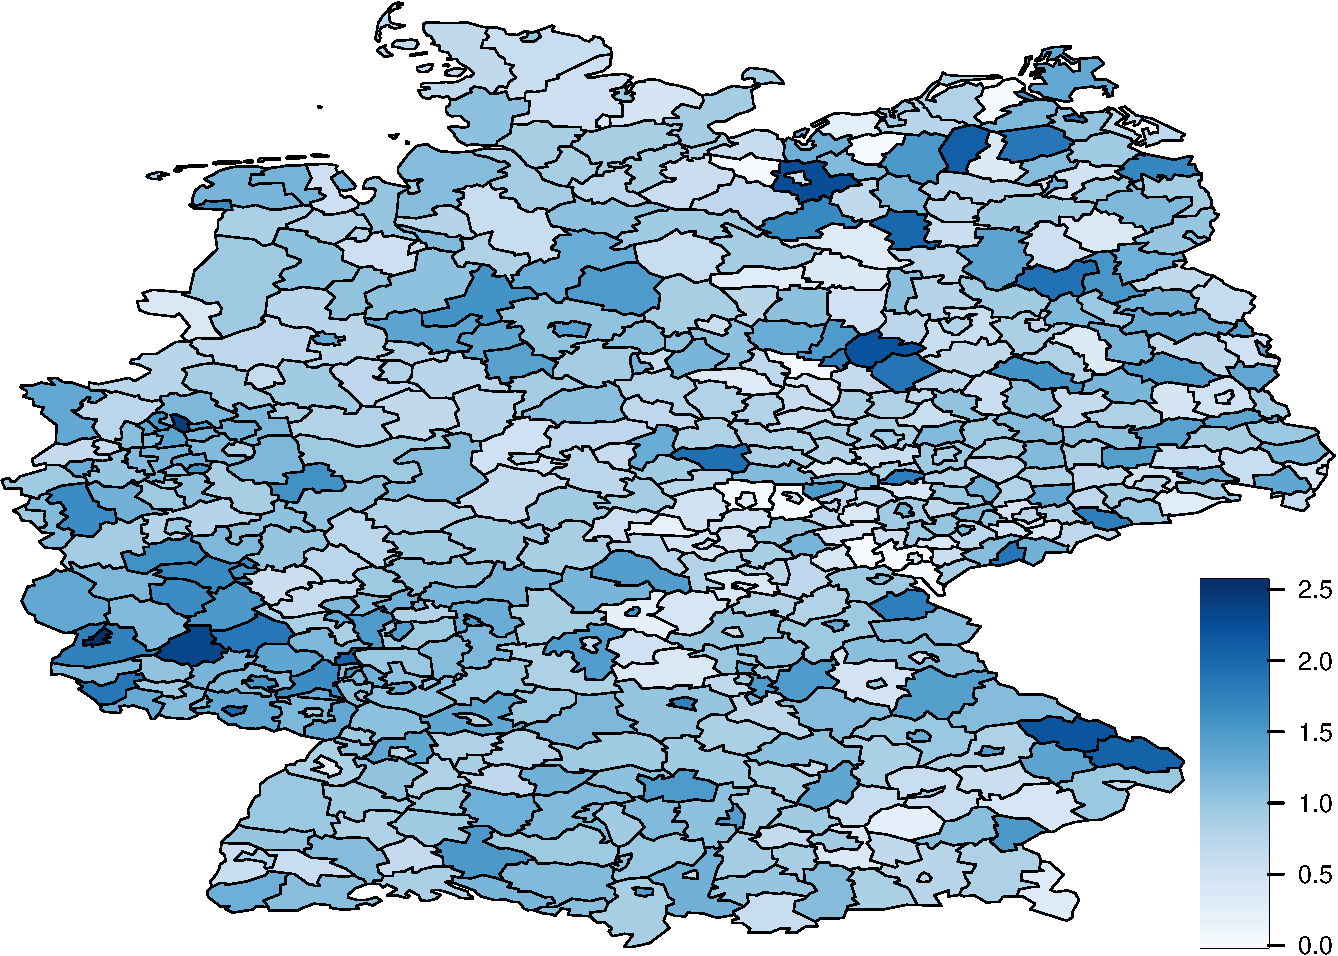
\includegraphics[width=1\linewidth]{Part3_Spatial_files/figure-beamer/unnamed-chunk-3-1} \end{center}

\end{col}

\end{cols}

\textbf{Observed response(s)}:

\begin{itemize}
\tightlist
\item
  Measurement over each grid cell (e.g.~number of individuals in cell;
  rainfall in province)
\end{itemize}
\end{frame}

\begin{frame}{Continuous Space: Geostatistics}
\protect\hypertarget{continuous-space-geostatistics}{}
\begin{cols}

\begin{col}{0.45\textwidth}

\begin{itemize}
\item
  phenomenon that is continuous in space
\item
  examples: nutrient levels in soil, salinity in the sea
\item
  measurements at a given set of locations that are determined by
  surveyor
\end{itemize}

\end{col}

\begin{col}{0.05\textwidth}
~

\end{col}

\begin{col}{0.55\textwidth}

\begin{center}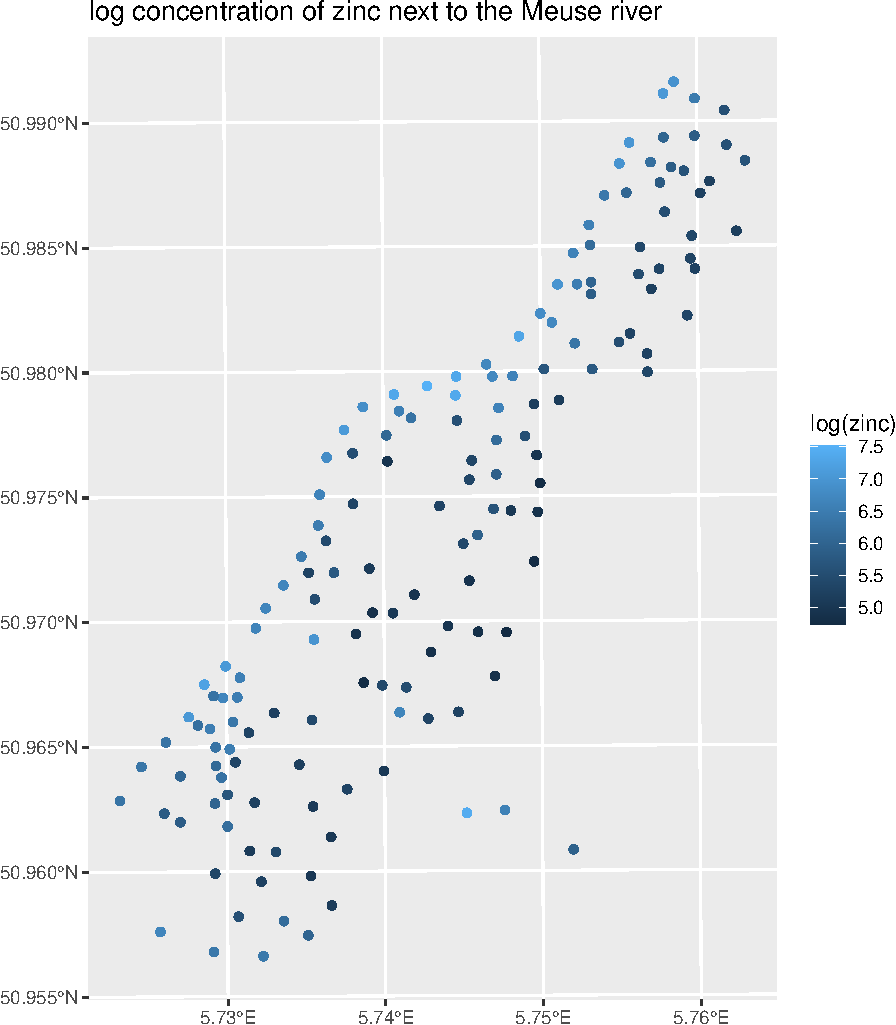
\includegraphics[width=0.8\linewidth]{Part3_Spatial_files/figure-beamer/unnamed-chunk-4-1} \end{center}

\end{col}

\end{cols}

\textbf{Observed response(s)}:

\begin{itemize}
\tightlist
\item
  measurement(s) taken at given locations
\end{itemize}
\end{frame}

\begin{frame}{Continuous Space: Point Process}
\protect\hypertarget{continuous-space-point-process}{}
\begin{cols}

\begin{col}{0.45\textwidth}

\begin{itemize}
\item
  locations of objects (individuals) in space (typically 2D)
\item
  examples: locations of trees in a forest, groups of animals
\end{itemize}

\end{col}

\begin{col}{0.05\textwidth}
~

\end{col}

\begin{col}{0.55\textwidth}

\begin{center}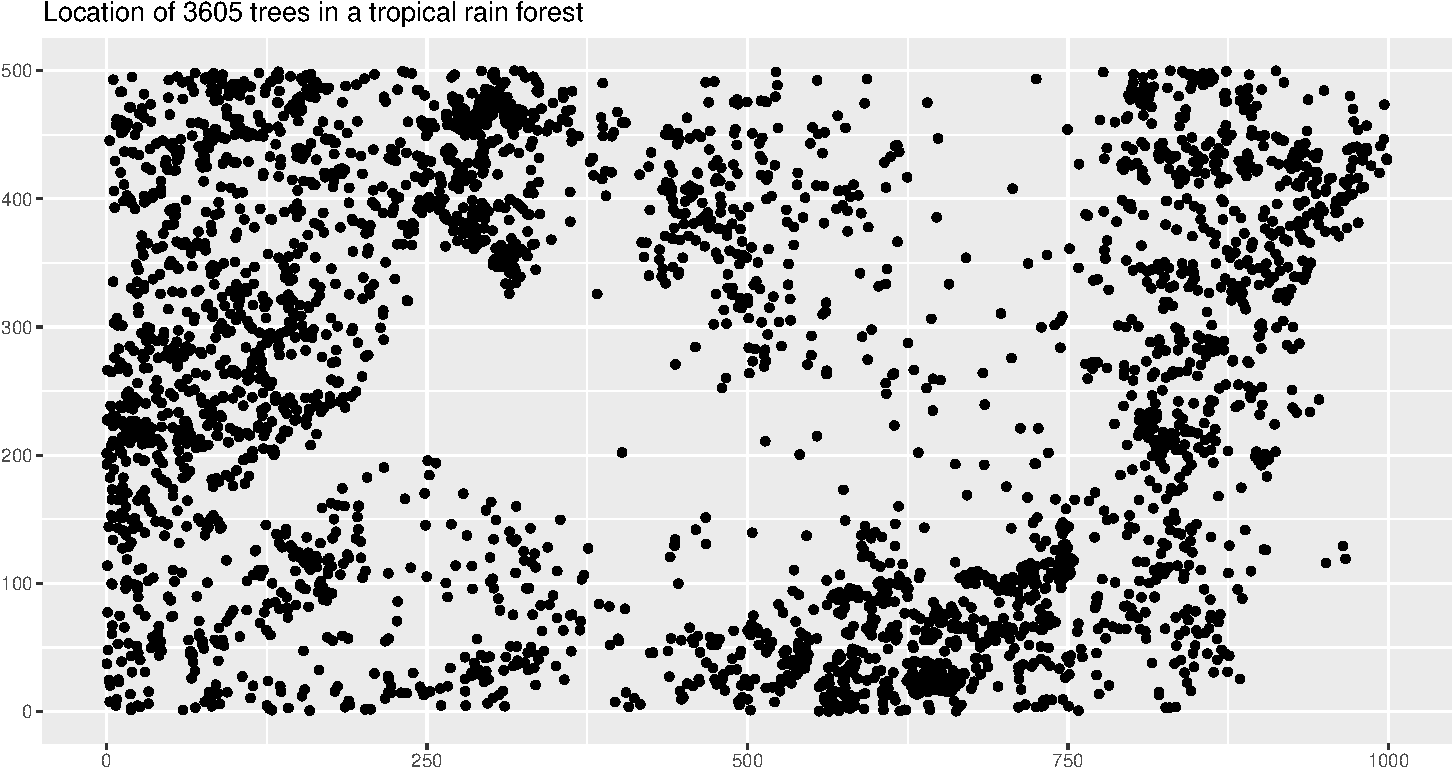
\includegraphics[width=0.8\linewidth]{Part3_Spatial_files/figure-beamer/unnamed-chunk-5-1} \end{center}

\end{col}

\end{cols}

\textbf{Observed response(s)}:

\begin{itemize}
\item
  \(x,y\) coordinates of points (individuals/groups)
\item
  maybe also properties of individuals/groups (``marks'')
\end{itemize}
\end{frame}

\hypertarget{gaussian-random-field-models}{%
\section{Gaussian Random Field
models}\label{gaussian-random-field-models}}

\begin{frame}{Gaussian Random fields}
\protect\hypertarget{gaussian-random-fields}{}
\textbf{Definition}:A random function \(u(x):R^d\rightarrow R\) is a
Gaussian random field if for any finite collection of locations,
\((x_1,\dots, x_n)\), \(x_i\in R^d\), the joint distribution of
\({\bf u} = (u(x_1),\dots, u(x_n))\) is \({\bf u} \sim N(0, \Sigma)\),
and

\[
\begin{aligned}
E(u(x)) = 0, &\\ 
Cov(u(x), u(x')) = R(x, x'), && \Sigma_{ij} = R(x_i, x_j)
\end{aligned}
\]

for some expectation function \(\mu(\cdot)\) and positive definite
covariance function \(R(\cdot, \cdot)\). \(\Sigma\) is the covariance
matrix for the specific location collection.
\end{frame}

\begin{frame}{Example}
\protect\hypertarget{example}{}
\begin{center}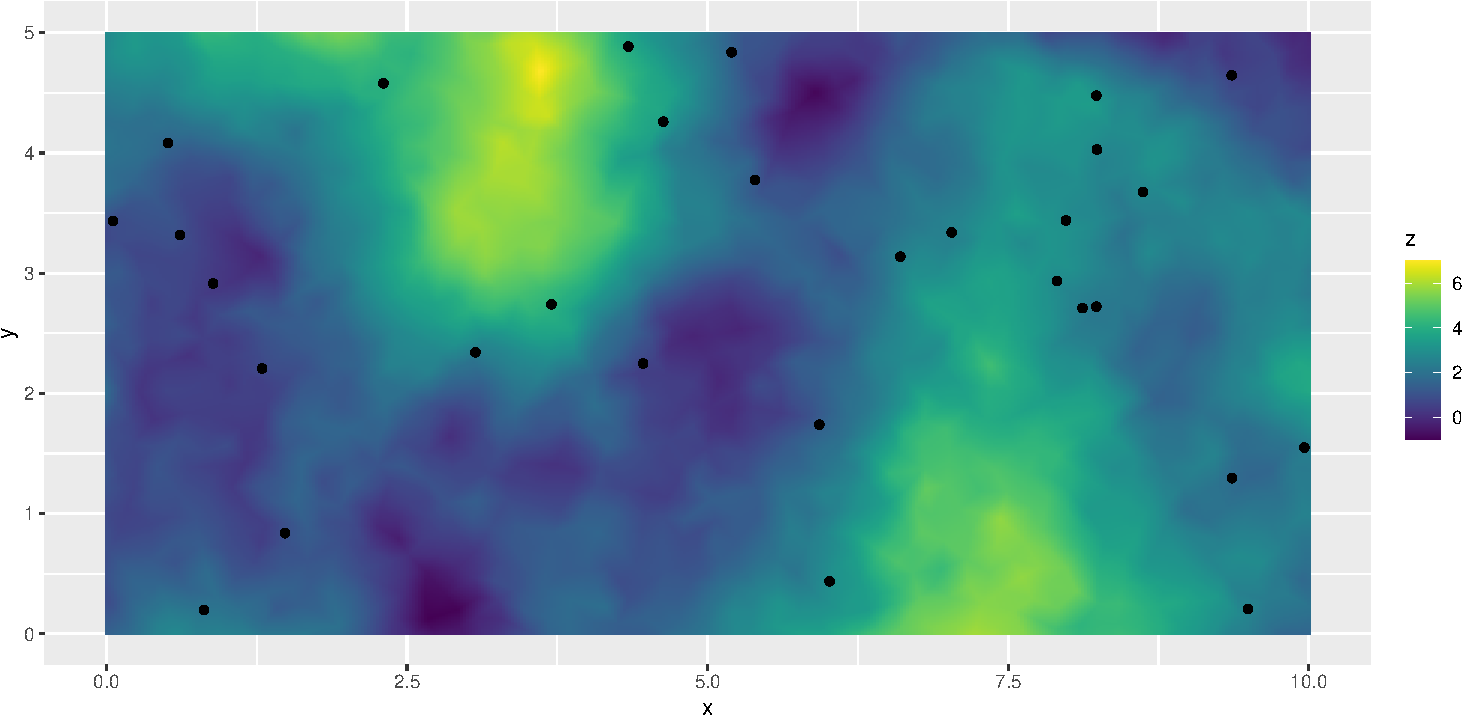
\includegraphics[width=0.6\linewidth]{Part3_Spatial_files/figure-beamer/unnamed-chunk-6-1} \end{center}
\end{frame}

\begin{frame}{Gaussian Random field}
\protect\hypertarget{gaussian-random-field}{}
GRF are a very popular model

\begin{itemize}
\item
  Flexible and easy to use
\item
  Can be part of the latent Gaussian field in a LGM
\end{itemize}

However:

\begin{itemize}
\item
  \textbf{computationally inefficient} (the precision matrix is dense)
\item
  not flexible enough (complicated boundary, barrier,\ldots)
\end{itemize}
\end{frame}

\hypertarget{the-spde-approach}{%
\section{The SPDE approach}\label{the-spde-approach}}

\begin{frame}{The SPDE approach}
\protect\hypertarget{the-spde-approach-1}{}
\begin{itemize}
\item
  Matern fields can be seen as solution to a PDE
\item
  Using finite element methods such solution can be represented using a
  GRMF\\
  \strut \\
\end{itemize}

\begin{center}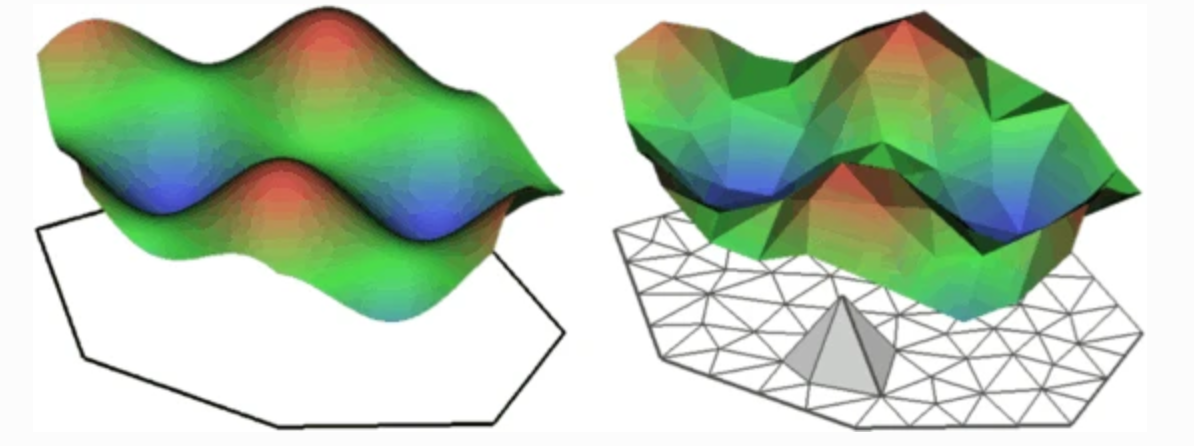
\includegraphics[width=0.7\linewidth]{graphics/spde} \end{center}
\end{frame}

\begin{frame}[fragile]{Advantages of the SPDE approach}
\protect\hypertarget{advantages-of-the-spde-approach}{}
\begin{itemize}
\item
  Computationally fast
\item
  Allows for flexible modeling

  \begin{itemize}
  \item
    non-stationary models (anisotropy)
  \item
    models on a sphere
  \item
    non separable models
  \end{itemize}
\end{itemize}

\begin{center}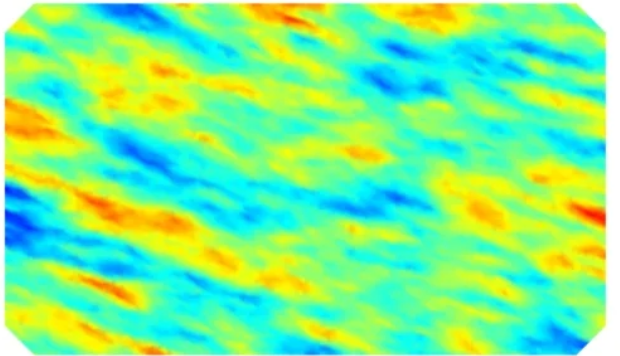
\includegraphics[width=0.29\linewidth,height=0.2\textheight]{graphics/fig1} 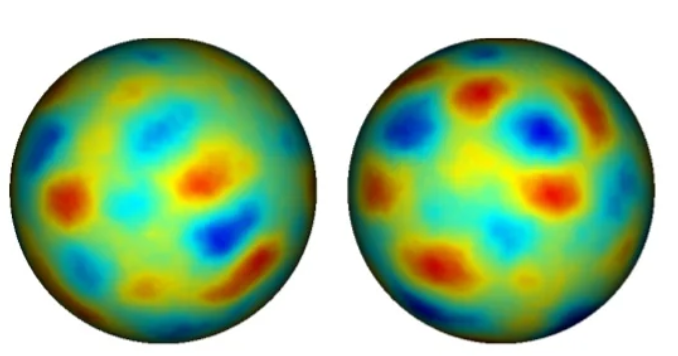
\includegraphics[width=0.29\linewidth,height=0.2\textheight]{graphics/fig2} \end{center}

All these models (and my more) can be fitted with \texttt{R-INLA} and
\texttt{inlabru}
\end{frame}

\begin{frame}{Learning about the SPDE approach}
\protect\hypertarget{learning-about-the-spde-approach}{}
\begin{itemize}
\item
  F. Lindgren, H. Rue, and J. Lindström. \emph{An explicit link between
  Gaussian fields and Gaussian Markov random fields: The SPDE approach
  (with discussion)}. In: Journal of the Royal Statistical Society,
  Series B 73.4 (2011), pp.~423--498.
\item
  H. Bakka, H. Rue, G. A. Fuglstad, A. Riebler, D. Bolin, J. Illian, E.
  Krainski, D. Simpson, and F. Lindgren. \emph{Spatial modelling with
  R-INLA: A review}. In: WIREs Computational Statistics 10:e1443.6
  (2018). (Invited extended review). DOI: 10.1002/wics.1443.
\item
  E. T. Krainski, V. Gómez-Rubio, H. Bakka, A. Lenzi, D. Castro-Camilio,
  D. Simpson, F. Lindgren, and H. Rue. \emph{Advanced Spatial Modeling
  with Stochastic Partial Differential Equations using R and INLA}.
  Github version \url{www.r-inla.org/spde-book}. CRC press, Dec.~20
\end{itemize}
\end{frame}

\hypertarget{fitting-spatial-models}{%
\section{Fitting spatial models}\label{fitting-spatial-models}}

\begin{frame}{Example: Meuse Data}
\protect\hypertarget{example-meuse-data}{}
Measures of zinc concentration.

\begin{center}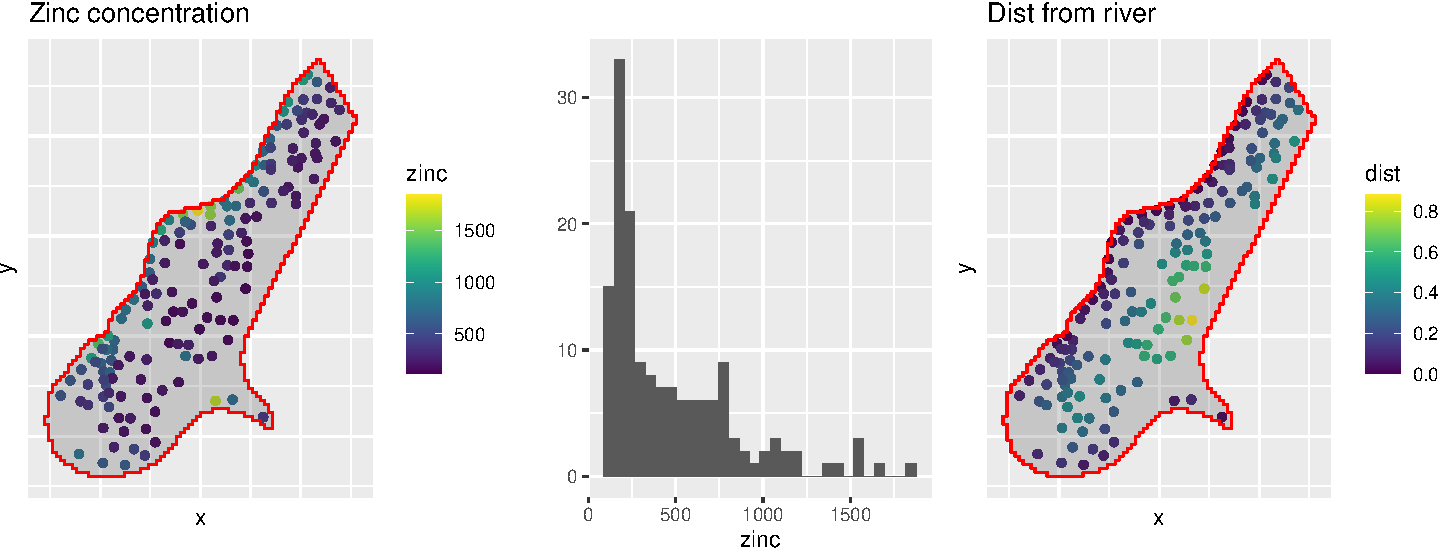
\includegraphics[width=0.6\linewidth,height=0.5\textheight]{Part3_Spatial_files/figure-beamer/unnamed-chunk-9-1} \end{center}
\end{frame}

\begin{frame}{The model}
\protect\hypertarget{the-model}{}
\[
\begin{aligned}
\log(Y(s)) &\sim \mathcal{N}(\eta(s),\sigma^2_y)\\
\eta(s)& = \alpha + \beta\ x(s) + u(s)\\
\end{aligned}
\]

where

\begin{itemize}
\item
  \(Y(s)\) is the measure of zinc in location \(s\)
\item
  \(\alpha\) a common intercept
\item
  \(\beta\) a model parameter
\item
  \(x(s)\) distance from the river at location \(s\)
\item
  \(u(s)\) the Matern Gaussian field
\end{itemize}
\end{frame}

\begin{frame}{Step 1: Define the SPDE representation}
\protect\hypertarget{step-1-define-the-spde-representation}{}
\begin{itemize}
\item
  The mesh
\item
  The SPDE model
\end{itemize}
\end{frame}

\begin{frame}[fragile]{Define the SPDE representation: The mesh}
\protect\hypertarget{define-the-spde-representation-the-mesh}{}
\begin{enumerate}
\tightlist
\item
  Define the mesh \small
\end{enumerate}

\begin{Shaded}
\begin{Highlighting}[]
\NormalTok{mesh }\OtherTok{\textless{}{-}} \FunctionTok{inla.mesh.2d}\NormalTok{(}\AttributeTok{loc.domain =} \FunctionTok{cbind}\NormalTok{(meuse}\SpecialCharTok{$}\NormalTok{x, meuse}\SpecialCharTok{$}\NormalTok{y), }
                     \AttributeTok{max.edge =} \FunctionTok{c}\NormalTok{(}\DecValTok{150}\NormalTok{, }\DecValTok{500}\NormalTok{),}
                     \AttributeTok{offset =} \FunctionTok{c}\NormalTok{(}\DecValTok{100}\NormalTok{, }\DecValTok{250}\NormalTok{) )}
\end{Highlighting}
\end{Shaded}

\begin{center}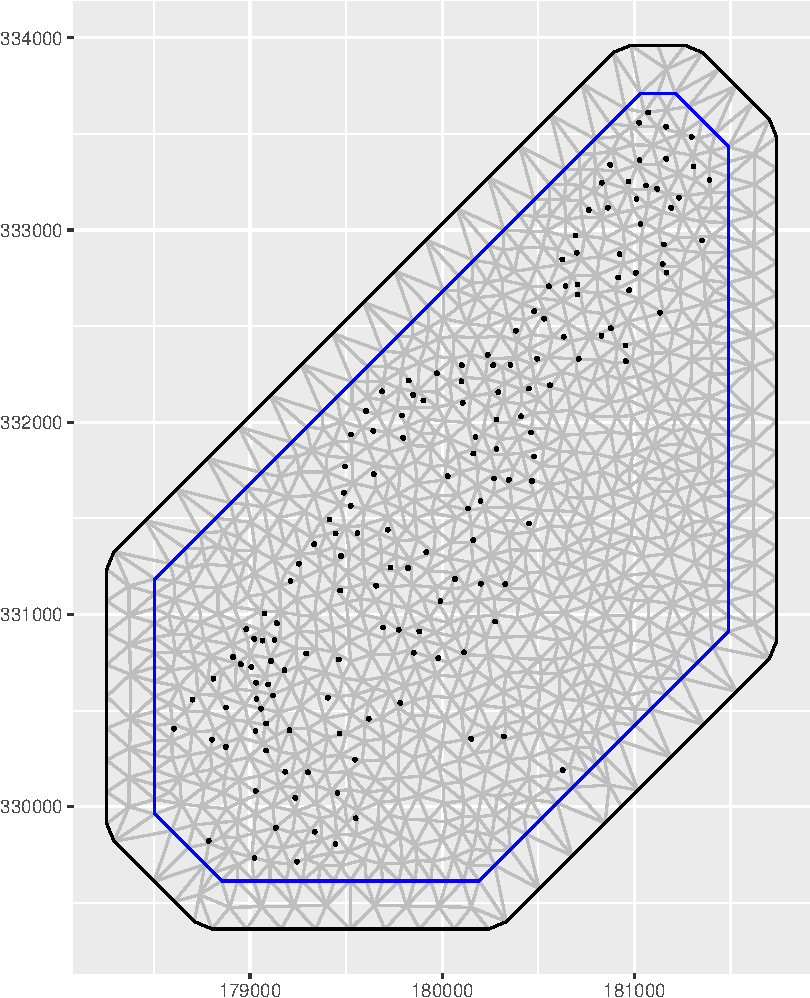
\includegraphics[width=0.4\linewidth]{Part3_Spatial_files/figure-beamer/unnamed-chunk-11-1} \end{center}
\normalsize
\end{frame}

\begin{frame}{Define the SPDE representation: The mesh}
\protect\hypertarget{define-the-spde-representation-the-mesh-1}{}
\footnotesize

\begin{itemize}
\item
  All random field models need to be discretised for practical
  calculations.
\item
  The SPDE models were developed to provide a consistent model
  definition across a range of discretisations.
\item
  We use finite element methods with local, piecewise linear basis
  functions defined on a triangulation of a region of space containing
  the domain of interest.
\item
  Deviation from stationarity is generated near the boundary of the
  region.
\item
  The choice of region and choice of triangulation affects the numerical
  accuracy.
\end{itemize}

\pause

Two separate issues:

\begin{itemize}
\item
  Continuous space with bounded domain: Boundary effect
\item
  Discretised model: Numerical accuracy
\end{itemize}

Sometimes the boundary effect may be desireable.

\normalsize
\end{frame}

\begin{frame}{Define the SPDE representation: The mesh}
\protect\hypertarget{define-the-spde-representation-the-mesh-2}{}
\begin{itemize}
\item
  Too fine meshes \(\rightarrow\) heavy computation
\item
  Too coarse mesh \(\rightarrow\) not accurate enought
\end{itemize}
\end{frame}

\begin{frame}[fragile]{Some guidelines}
\protect\hypertarget{some-guidelines}{}
\begin{itemize}
\item
  Create triangulation meshes with \texttt{inla.mesh.2d()}
\item
  Move undesired boundary effects away from the domain of interest by
  extending to a smooth external boundary
  (\texttt{inla.nonconvex.hull(loc,\ convex)}, \texttt{convex} \(\geq\)
  correlation range)
\item
  Use a coarser resolution in the extension to reduce computational cost
  (\texttt{max.edge=c(inner,\ outer)})
\item
  Use a fine resolution (subject to available computational resources)
  for the domain of interest (inner correlation range) and filter out
  small input point clusters
  (\texttt{0\ \textless{}\ cutoff\ \textless{}\ inner})
\item
  Coastlines and similar can be added to the domain specification in
  \texttt{inla.mesh.2d()}
\end{itemize}
\end{frame}

\begin{frame}[fragile]{Define the SPDE representation: The mesh}
\protect\hypertarget{define-the-spde-representation-the-mesh-3}{}
\small

\begin{Shaded}
\begin{Highlighting}[]
\NormalTok{mesh1 }\OtherTok{=} \FunctionTok{inla.mesh.2d}\NormalTok{(}\AttributeTok{loc.domain =} \FunctionTok{cbind}\NormalTok{(meuse}\SpecialCharTok{$}\NormalTok{x, meuse}\SpecialCharTok{$}\NormalTok{y), }
                     \AttributeTok{max.edge =} \DecValTok{350}\NormalTok{,}
                     \AttributeTok{offset =} \DecValTok{10}\NormalTok{)}

\NormalTok{mesh2 }\OtherTok{=} \FunctionTok{inla.mesh.2d}\NormalTok{(}\AttributeTok{loc.domain =} \FunctionTok{cbind}\NormalTok{(meuse}\SpecialCharTok{$}\NormalTok{x, meuse}\SpecialCharTok{$}\NormalTok{y), }
                     \AttributeTok{max.edge =} \FunctionTok{c}\NormalTok{(}\DecValTok{150}\NormalTok{, }\DecValTok{500}\NormalTok{),}
                     \AttributeTok{cutoff =} \DecValTok{100}\NormalTok{,}
                     \AttributeTok{offset =} \FunctionTok{c}\NormalTok{(}\DecValTok{100}\NormalTok{, }\DecValTok{550}\NormalTok{) )}
\end{Highlighting}
\end{Shaded}

\begin{center}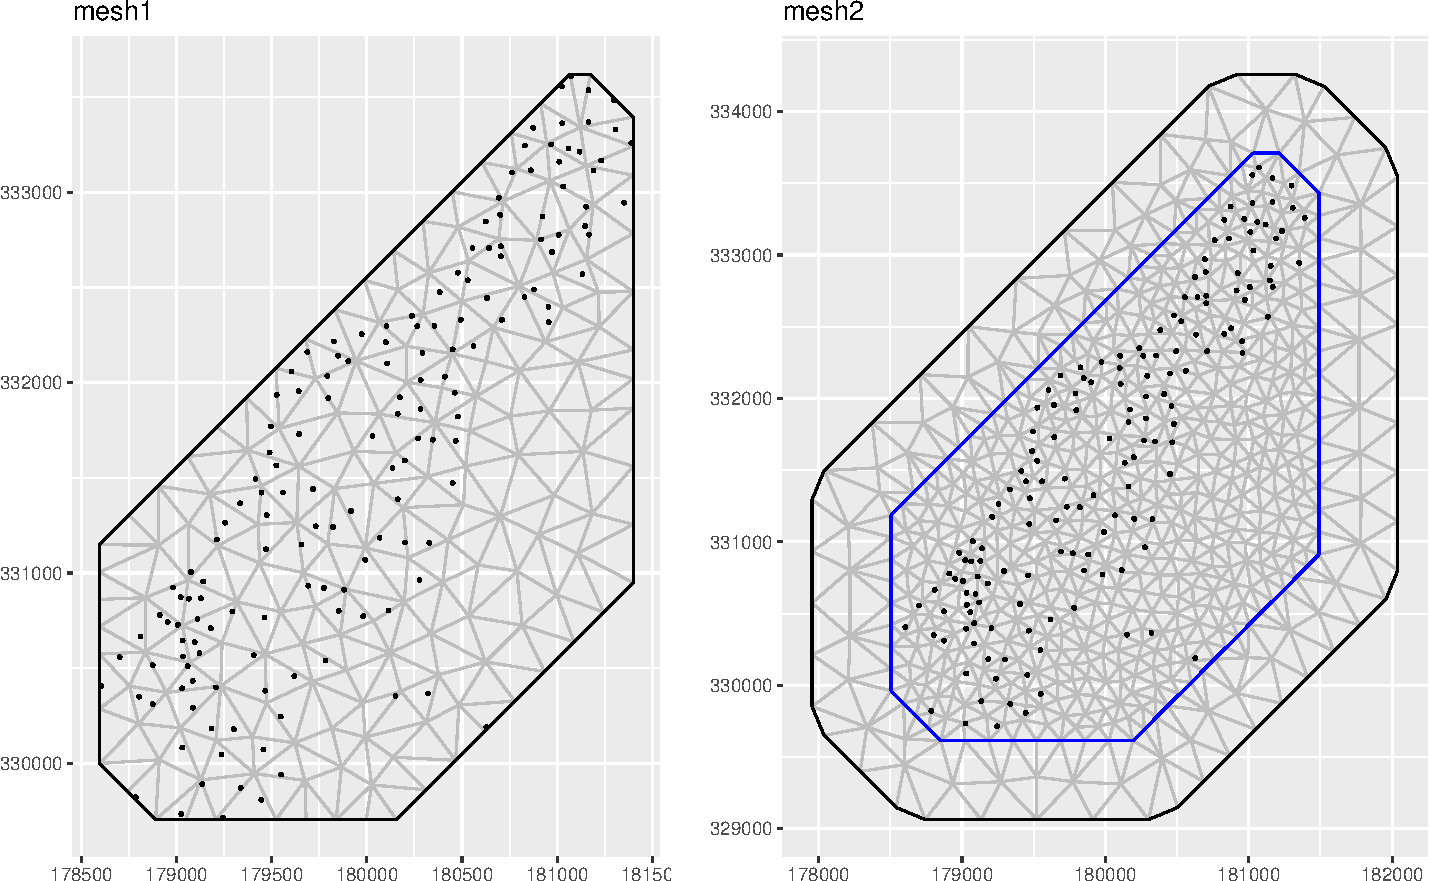
\includegraphics[width=0.6\linewidth]{Part3_Spatial_files/figure-beamer/unnamed-chunk-13-1} \end{center}
\normalsize
\end{frame}

\begin{frame}[fragile]{Define the SPDE representation: The SPDE model}
\protect\hypertarget{define-the-spde-representation-the-spde-model}{}
\small

\begin{Shaded}
\begin{Highlighting}[]
\NormalTok{meuse.spde }\OtherTok{\textless{}{-}} \FunctionTok{inla.spde2.pcmatern}\NormalTok{(}\AttributeTok{mesh =}\NormalTok{ mesh,}
                                  \AttributeTok{prior.sigma =} \FunctionTok{c}\NormalTok{(}\DecValTok{1}\NormalTok{, }\FloatTok{0.1}\NormalTok{),}
                                  \AttributeTok{prior.range =} \FunctionTok{c}\NormalTok{(}\DecValTok{1000}\NormalTok{, }\FloatTok{0.5}\NormalTok{))}
\end{Highlighting}
\end{Shaded}

\normalsize

PC-priors for the range \(\rho\) and the standard deviarion \(\sigma\)

\begin{itemize}
\item
  Define the prior for the range
  \texttt{prior.range\ \ =\ (range0,Prange)}
  \(\text{Prob}(\rho<\rho_0) = p_{\rho}\)
\item
  Define the prior for the range
  \texttt{prior.sigma\ \ =\ (sigma0,Psigma)}
  \(\text{Prob}(\sigma>\sigma_0) = p_{\sigma}\)
\end{itemize}
\end{frame}

\begin{frame}[fragile]{Run the model \texttt{inlabru}}
\protect\hypertarget{run-the-model-inlabru}{}
\tiny

\begin{Shaded}
\begin{Highlighting}[]
\CommentTok{\# create a spatial object}
\FunctionTok{coordinates}\NormalTok{(meuse) }\OtherTok{=} \FunctionTok{c}\NormalTok{(}\StringTok{"x"}\NormalTok{,}\StringTok{"y"}\NormalTok{)}
\CommentTok{\#  covariate values}
\NormalTok{dist\_SPDE }\OtherTok{=} \FunctionTok{SpatialPixelsDataFrame}\NormalTok{(data}\SpecialCharTok{$}\NormalTok{dist\_raster[,}\FunctionTok{c}\NormalTok{(}\DecValTok{1}\NormalTok{,}\DecValTok{2}\NormalTok{)], }
                                  \AttributeTok{data =} \FunctionTok{data.frame}\NormalTok{(}\AttributeTok{dist =}\NormalTok{ data}\SpecialCharTok{$}\NormalTok{dist\_raster[,}\DecValTok{3}\NormalTok{]))}
\CommentTok{\# model components}
\NormalTok{cmp }\OtherTok{=}  \ErrorTok{\textasciitilde{}} \FunctionTok{Intercept}\NormalTok{(}\DecValTok{1}\NormalTok{) }\SpecialCharTok{+} \FunctionTok{dist}\NormalTok{(dist\_SPDE, }\AttributeTok{model =} \StringTok{"linear"}\NormalTok{) }\SpecialCharTok{+} 
  \FunctionTok{spde}\NormalTok{(coordinates, }\AttributeTok{model =}\NormalTok{ meuse.spde)}
\CommentTok{\# define likelihood}
\NormalTok{lik }\OtherTok{=} \FunctionTok{like}\NormalTok{(}\AttributeTok{formula =}\NormalTok{ Y }\SpecialCharTok{\textasciitilde{}}\NormalTok{ Intercept }\SpecialCharTok{+}\NormalTok{ dist }\SpecialCharTok{+}\NormalTok{   spde,}
           \AttributeTok{family =} \StringTok{"gaussian"}\NormalTok{,}
           \AttributeTok{data  =}\NormalTok{ meuse)}
\CommentTok{\#fit the model}
\NormalTok{fit }\OtherTok{\textless{}{-}} \FunctionTok{bru}\NormalTok{(cmp, lik)}
\CommentTok{\# define prediction area}
\NormalTok{pix }\OtherTok{\textless{}{-}} \FunctionTok{pixels}\NormalTok{(mesh, }\AttributeTok{nx =} \DecValTok{200}\NormalTok{, }\AttributeTok{ny =} \DecValTok{200}\NormalTok{, }\AttributeTok{mask =}\NormalTok{ boundary)}
\CommentTok{\# generate predictions}
\NormalTok{pred }\OtherTok{=} \FunctionTok{predict}\NormalTok{(fit, pix, }\SpecialCharTok{\textasciitilde{}} \FunctionTok{data.frame}\NormalTok{(}
                                      \AttributeTok{spde =}\NormalTok{ spde,}
                                      \AttributeTok{logscale =}\NormalTok{ Intercept }\SpecialCharTok{+}\NormalTok{ dist }\SpecialCharTok{+}\NormalTok{ spde,}
                                      \AttributeTok{naturalscale =} \FunctionTok{exp}\NormalTok{(Intercept }\SpecialCharTok{+}\NormalTok{ dist }\SpecialCharTok{+}\NormalTok{ spde)))}
\end{Highlighting}
\end{Shaded}
\end{frame}

\begin{frame}[fragile]{Notes!}
\protect\hypertarget{notes}{}
\begin{itemize}
\item
  The data are a spatial object!
\item
  For prediction, the covariates are stored in a
  \texttt{SpatialPixelsDataFrame} and need to cover all the mesh nodes
\end{itemize}
\end{frame}

\begin{frame}{Predictions: The SPDE field}
\protect\hypertarget{predictions-the-spde-field}{}
\begin{center}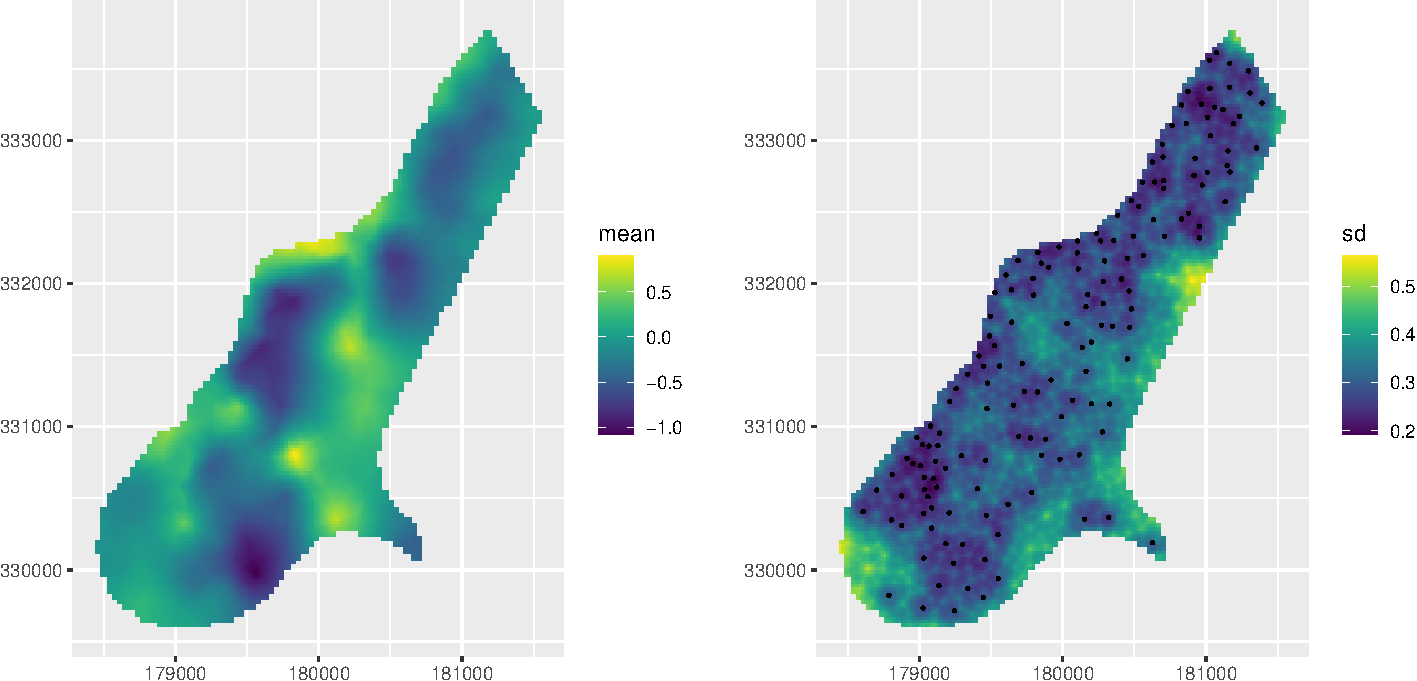
\includegraphics[width=0.8\linewidth]{Part3_Spatial_files/figure-beamer/unnamed-chunk-19-1} \end{center}
\end{frame}

\begin{frame}{Predictions: The log concentrations}
\protect\hypertarget{predictions-the-log-concentrations}{}
\begin{center}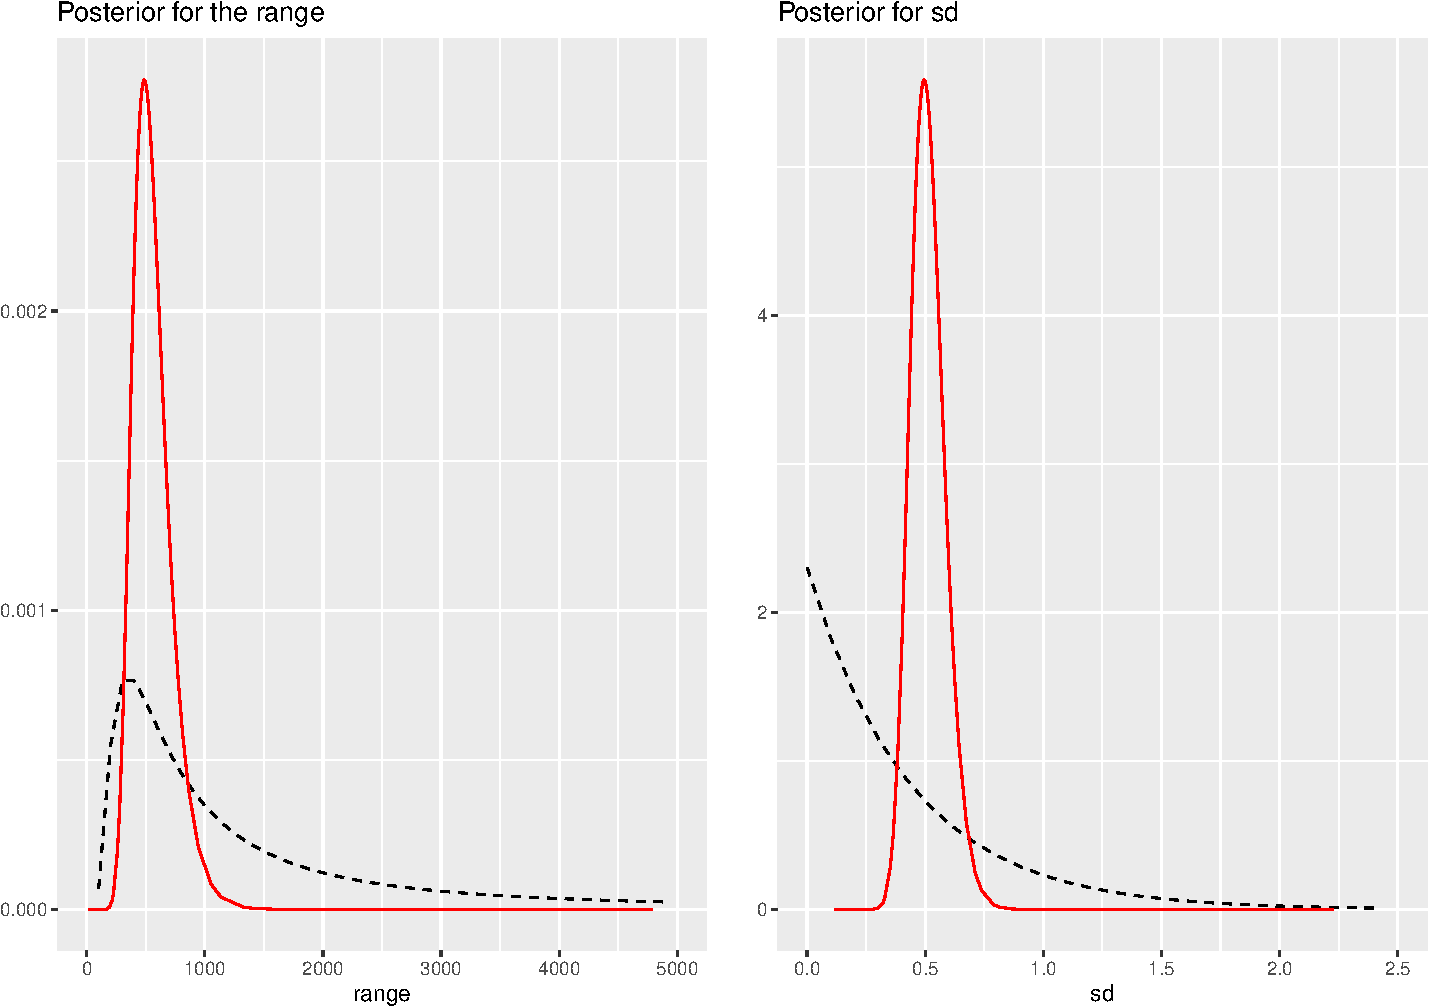
\includegraphics[width=0.8\linewidth]{Part3_Spatial_files/figure-beamer/unnamed-chunk-20-1} \end{center}
\end{frame}

\begin{frame}{Predictions: The concentrations}
\protect\hypertarget{predictions-the-concentrations}{}
\begin{center}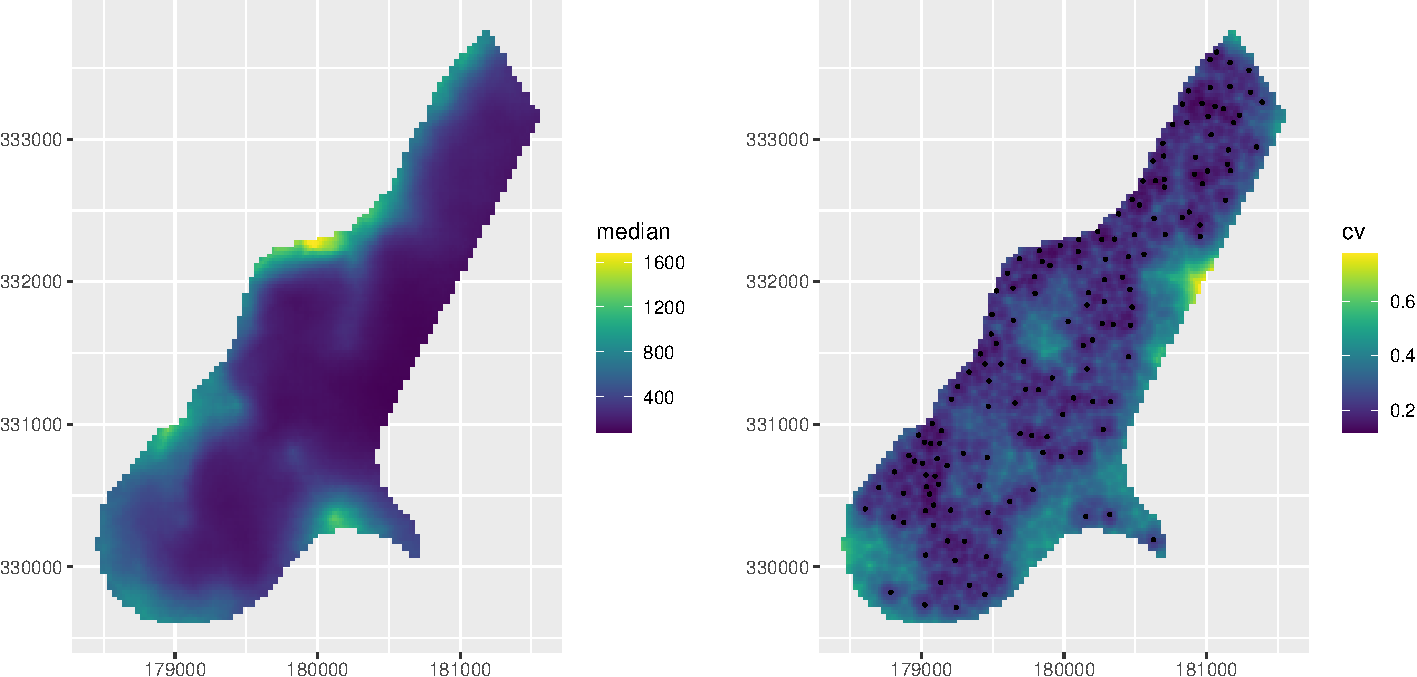
\includegraphics[width=0.8\linewidth]{Part3_Spatial_files/figure-beamer/unnamed-chunk-21-1} \end{center}
\end{frame}

\begin{frame}[fragile]{Same in plain \texttt{INLA} (1)}
\protect\hypertarget{same-in-plain-inla-1}{}
\tiny

\begin{Shaded}
\begin{Highlighting}[]
\NormalTok{A.meuse }\OtherTok{\textless{}{-}} \FunctionTok{inla.spde.make.A}\NormalTok{(}\AttributeTok{mesh =}\NormalTok{ mesh, }\AttributeTok{loc =} \FunctionTok{coordinates}\NormalTok{(meuse))}
\NormalTok{s.index }\OtherTok{\textless{}{-}} \FunctionTok{inla.spde.make.index}\NormalTok{(}\AttributeTok{name =} \StringTok{"spatial.field"}\NormalTok{,}
  \AttributeTok{n.spde =}\NormalTok{ meuse.spde}\SpecialCharTok{$}\NormalTok{n.spde)}

\CommentTok{\#Create data structure}
\NormalTok{meuse.stack }\OtherTok{\textless{}{-}} \FunctionTok{inla.stack}\NormalTok{(}\AttributeTok{data  =} \FunctionTok{list}\NormalTok{(}\AttributeTok{zinc =}\NormalTok{ meuse}\SpecialCharTok{$}\NormalTok{zinc),}
  \AttributeTok{A =} \FunctionTok{list}\NormalTok{(A.meuse, }\DecValTok{1}\NormalTok{),}
  \AttributeTok{effects =} \FunctionTok{list}\NormalTok{(}\FunctionTok{c}\NormalTok{(s.index, }\FunctionTok{list}\NormalTok{(}\AttributeTok{Intercept =} \DecValTok{1}\NormalTok{)),}
    \FunctionTok{list}\NormalTok{(}\AttributeTok{dist =}\NormalTok{ meuse}\SpecialCharTok{$}\NormalTok{dist)),}
  \AttributeTok{tag =} \StringTok{"meuse.data"}\NormalTok{)}

\FunctionTok{data}\NormalTok{(meuse.grid)}
\FunctionTok{coordinates}\NormalTok{(meuse.grid) }\OtherTok{=} \ErrorTok{\textasciitilde{}}\NormalTok{x}\SpecialCharTok{+}\NormalTok{y}
\FunctionTok{gridded}\NormalTok{(meuse.grid) }\OtherTok{=} \ConstantTok{TRUE}

\CommentTok{\#Create data structure for prediction}
\NormalTok{A.pred }\OtherTok{\textless{}{-}} \FunctionTok{inla.spde.make.A}\NormalTok{(}\AttributeTok{mesh =}\NormalTok{ mesh, }\AttributeTok{loc =} \FunctionTok{coordinates}\NormalTok{(meuse.grid))}
\NormalTok{meuse.stack.pred }\OtherTok{\textless{}{-}} \FunctionTok{inla.stack}\NormalTok{(}\AttributeTok{data =} \FunctionTok{list}\NormalTok{(}\AttributeTok{zinc =} \ConstantTok{NA}\NormalTok{),}
  \AttributeTok{A =} \FunctionTok{list}\NormalTok{(A.pred, }\DecValTok{1}\NormalTok{),}
  \AttributeTok{effects =} \FunctionTok{list}\NormalTok{(}\FunctionTok{c}\NormalTok{(s.index, }\FunctionTok{list}\NormalTok{ (}\AttributeTok{Intercept =} \DecValTok{1}\NormalTok{)),}
    \FunctionTok{list}\NormalTok{(}\AttributeTok{dist =}\NormalTok{ meuse.grid}\SpecialCharTok{$}\NormalTok{dist)),}
  \AttributeTok{tag =} \StringTok{"meuse.pred"}\NormalTok{)}

\CommentTok{\#Join stack}
\NormalTok{join.stack }\OtherTok{\textless{}{-}} \FunctionTok{inla.stack}\NormalTok{(meuse.stack, meuse.stack.pred)}
\end{Highlighting}
\end{Shaded}
\end{frame}

\begin{frame}[fragile]{Same in plain \texttt{INLA} (2)}
\protect\hypertarget{same-in-plain-inla-2}{}
\tiny

\begin{Shaded}
\begin{Highlighting}[]
\CommentTok{\#Fit model}
\NormalTok{form }\OtherTok{\textless{}{-}} \FunctionTok{log}\NormalTok{(zinc) }\SpecialCharTok{\textasciitilde{}} \SpecialCharTok{{-}}\DecValTok{1} \SpecialCharTok{+}\NormalTok{ Intercept }\SpecialCharTok{+}\NormalTok{ dist }\SpecialCharTok{+} \FunctionTok{f}\NormalTok{(spatial.field, }\AttributeTok{model =}\NormalTok{ spde)}

\NormalTok{m1 }\OtherTok{\textless{}{-}} \FunctionTok{inla}\NormalTok{(form, }\AttributeTok{data =} \FunctionTok{inla.stack.data}\NormalTok{(join.stack, }\AttributeTok{spde =}\NormalTok{ meuse.spde),}
  \AttributeTok{family =} \StringTok{"gaussian"}\NormalTok{,}
  \AttributeTok{control.predictor =} \FunctionTok{list}\NormalTok{(}\AttributeTok{A =} \FunctionTok{inla.stack.A}\NormalTok{(join.stack), }\AttributeTok{compute =} \ConstantTok{TRUE}\NormalTok{))}
\end{Highlighting}
\end{Shaded}

\normalsize

\textbf{Note}: We still have not compute predictions\ldots and this is
not too easy in plain \texttt{INLA}!!
\end{frame}

\begin{frame}[fragile]{When is \texttt{inlabru} easier to use}
\protect\hypertarget{when-is-inlabru-easier-to-use}{}
\begin{itemize}
\item
  spatial modeling.
\item
  point processes.
\item
  multiple likelihoods
\item
  when interested in spatial predictions
\end{itemize}

\pause

\begin{itemize}
\item
  \texttt{inlabru} is also useful if one has non-linearities in the
  predictor \(\eta\)

  \begin{itemize}
  \tightlist
  \item
    born for ecological models (for example transect sampling) but used
    also in other fields
  \end{itemize}
\end{itemize}

\pause

What cannot (at the moment ) be done with \texttt{inlabru}

\begin{itemize}
\tightlist
\item
  Survival models
\end{itemize}
\end{frame}

\hypertarget{space-time-modeling}{%
\section{Space-time Modeling}\label{space-time-modeling}}

\begin{frame}{Modeling PM10 concentration in Piemonte (Italy)}
\protect\hypertarget{modeling-pm10-concentration-in-piemonte-italy}{}
\begin{center}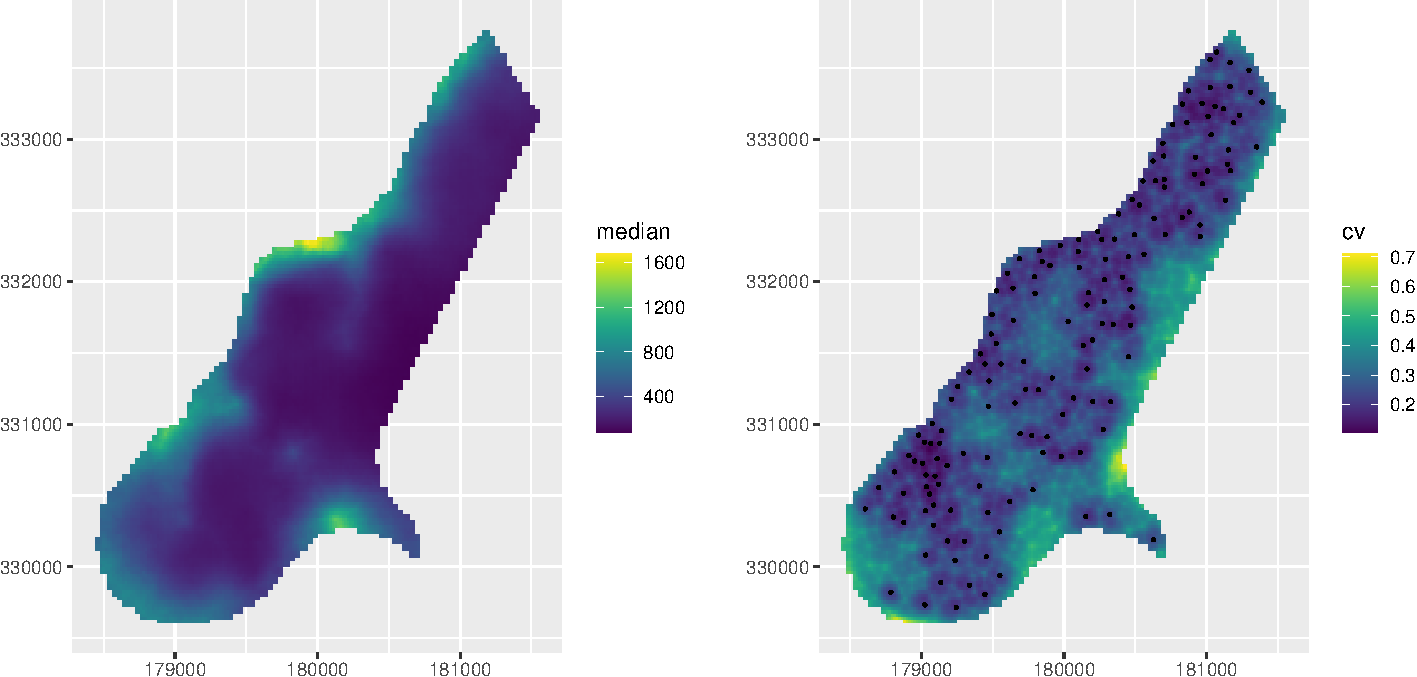
\includegraphics[width=0.9\linewidth]{Part3_Spatial_files/figure-beamer/unnamed-chunk-24-1} \end{center}
\end{frame}

\begin{frame}[fragile]{Modeling PM10 concentration in Piemonte (Italy)}
\protect\hypertarget{modeling-pm10-concentration-in-piemonte-italy-1}{}
Example from the Blangiardo \& Cameletti book but simplified! \tiny

\begin{verbatim}
##   Station.ID       Date   dem      x       y   WS   temp   HMIX PREC   EMI PM10
## 1          1 2005-10-01  95.2 469.45 4972.85 0.90 288.81 1294.6    0 26.05   28
## 2          2 2005-10-01 164.1 423.48 4950.69 0.82 288.67 1139.8    0 18.74   22
## 3          3 2005-10-01 242.9 490.71 4948.86 0.96 287.44 1404.0    0  6.28   17
## 4          4 2005-10-01 149.9 437.36 4973.34 1.17 288.63 1042.4    0 29.35   25
## 5          5 2005-10-01 405.0 426.44 5045.66 0.60 287.63 1038.7    0 32.19   20
##   time  logPM10
## 1    1 3.332205
## 2    1 3.091042
## 3    1 2.833213
## 4    1 3.218876
## 5    1 2.995732
\end{verbatim}

\normalsize
\end{frame}

\begin{frame}{The model}
\protect\hypertarget{the-model-1}{}
We model the log PM10 concentration:

\[
\begin{aligned}
y_{it}&\sim\mathcal{N}(\eta_it, \sigma^2_e)\\
\eta_{it}& = \alpha + \beta_1\text{dem}_i + \beta_2\text{temp}_{it} + \omega_{it}
\end{aligned}
\]

\begin{itemize}
\item
  \(y_{it}\) is the log-concentration at location \(i\) in time \(t\)
\item
  \(\alpha\) is an intercept
\item
  \(\beta_1\) and \(\beta_2\) parameters of altitude and temperature
\item
  \(\omega_{it}\) is the space-time residual
\end{itemize}
\end{frame}

\begin{frame}{Space time residual model}
\protect\hypertarget{space-time-residual-model}{}
A first order autoregressive process with spatially colored innovations

\[
\omega_{it}  = a \omega_{i(t-1)}+\xi_{it}
\]

\begin{itemize}
\item
  \(|a|<1\) parameter of the AR1 process
\item
  \(\xi_{it}\) is a zero mean, temporally independent, Gaussian field
  with
\end{itemize}

\[
\text{Cov}(\xi_{it},\xi_{ju})  =
\begin{cases}
 0 ,& \text{ if } t\neq u \\
 \mathcal{C}(h),&  \text{ if } t= u
 \end{cases}
\] - \(h\) distance between locations \(i\) and \(j\) -
\(\mathcal{C}(h)\) is a Matern correlation function
\end{frame}

\begin{frame}{Building the model: mesh}
\protect\hypertarget{building-the-model-mesh}{}
\begin{center}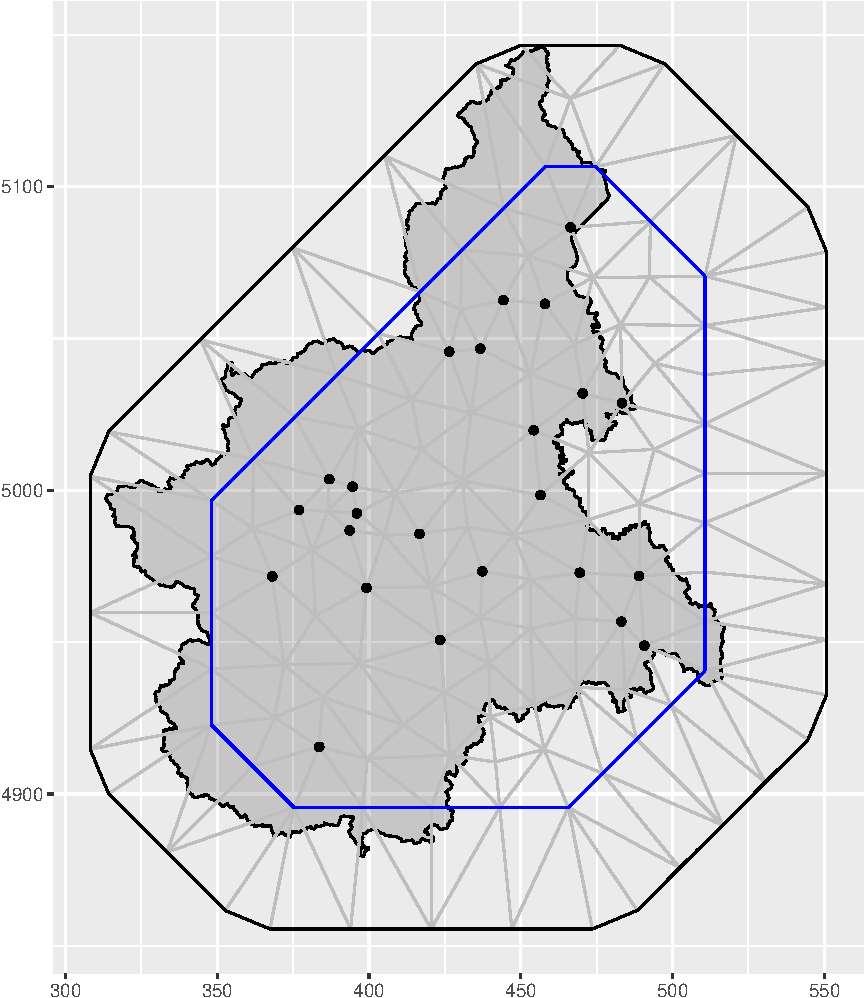
\includegraphics[width=0.6\linewidth]{Part3_Spatial_files/figure-beamer/unnamed-chunk-26-1} \end{center}
\end{frame}

\begin{frame}[fragile]{Building the model: Prior for the spde model}
\protect\hypertarget{building-the-model-prior-for-the-spde-model}{}
\small

\begin{Shaded}
\begin{Highlighting}[]
\NormalTok{spde }\OtherTok{=} \FunctionTok{inla.spde2.pcmatern}\NormalTok{(}\AttributeTok{mesh =}\NormalTok{ mesh,}
                           \AttributeTok{prior.range=}\FunctionTok{c}\NormalTok{(}\DecValTok{100}\NormalTok{,}\FloatTok{0.5}\NormalTok{), }
                           \AttributeTok{prior.sigma=}\FunctionTok{c}\NormalTok{(}\DecValTok{1}\NormalTok{,}\FloatTok{0.1}\NormalTok{)) }
\end{Highlighting}
\end{Shaded}

\normalsize

\begin{itemize}
\item
  \(\text{Prob}(\rho<100\text{ Km}) = 0.5\)
\item
  \(\text{Prob}(\sigma>1) = 0.1\)
\end{itemize}
\end{frame}

\begin{frame}[fragile]{Implement the model}
\protect\hypertarget{implement-the-model}{}
\small

\begin{Shaded}
\begin{Highlighting}[]
\CommentTok{\# make the data a spatial object}
\FunctionTok{coordinates}\NormalTok{(df) }\OtherTok{=} \FunctionTok{c}\NormalTok{(}\StringTok{"x"}\NormalTok{,}\StringTok{"y"}\NormalTok{)}

\CommentTok{\# model component}
\NormalTok{cmp  }\OtherTok{=} \ErrorTok{\textasciitilde{}} \FunctionTok{Intercept}\NormalTok{(}\DecValTok{1}\NormalTok{) }\SpecialCharTok{+} 
  \FunctionTok{SPDE}\NormalTok{(coordinates, }\AttributeTok{model =}\NormalTok{ spde,}
       \AttributeTok{group =}\NormalTok{ time, }\AttributeTok{control.group =} \FunctionTok{list}\NormalTok{(}\AttributeTok{model =} \StringTok{"ar1"}\NormalTok{)) }\SpecialCharTok{+}
  \FunctionTok{dem}\NormalTok{(dem, }\AttributeTok{model =} \StringTok{"linear"}\NormalTok{) }\SpecialCharTok{+} 
  \FunctionTok{temp}\NormalTok{(temp, }\AttributeTok{model =} \StringTok{"linear"}\NormalTok{)}

\CommentTok{\# likelihood}
\NormalTok{lik }\OtherTok{=} \FunctionTok{like}\NormalTok{(}\AttributeTok{formula =}\NormalTok{ logPM10 }\SpecialCharTok{\textasciitilde{}}\NormalTok{ Intercept }\SpecialCharTok{+}\NormalTok{ SPDE }\SpecialCharTok{+}\NormalTok{ dem }\SpecialCharTok{+}\NormalTok{ temp ,}
           \AttributeTok{family =} \StringTok{"gaussian"}\NormalTok{,}
           \AttributeTok{data =}\NormalTok{ df)}

\CommentTok{\# fit the model}
\NormalTok{fit }\OtherTok{=} \FunctionTok{bru}\NormalTok{(cmp, lik,}
          \AttributeTok{options =} \FunctionTok{list}\NormalTok{(}\AttributeTok{verbose =}\NormalTok{ F,}
                         \AttributeTok{bru\_max\_iter =} \DecValTok{1}\NormalTok{,}
                         \AttributeTok{inla.mode  =} \StringTok{"experimental"}\NormalTok{))}
\end{Highlighting}
\end{Shaded}
\end{frame}

\begin{frame}[fragile]{Model Parameters}
\protect\hypertarget{model-parameters}{}
Fixed effects: \tiny

\begin{verbatim}
##                    mean           sd   0.025quant  0.975quant
## Intercept -1.438049e+01 9.2184286118 -32.13870144 4.048280505
## dem       -7.283542e-04 0.0008432266  -0.00239864 0.000935377
## temp       6.250714e-02 0.0320763923  -0.00168185 0.124370511
\end{verbatim}

\normalsize

Hyperparameters of the random field: \tiny

\begin{verbatim}
##                                                mean          sd  0.025quant
## Precision for the Gaussian observations  41.8618738  7.23316236  29.3259934
## Range for SPDE                          129.1743804 16.95258105 101.0603416
## Stdev for SPDE                            0.7512039  0.09966426   0.5914011
## GroupRho for SPDE                         0.9105342  0.02594714   0.8555936
##                                          0.975quant
## Precision for the Gaussian observations  57.6623693
## Range for SPDE                          167.2435983
## Stdev for SPDE                            0.9798284
## GroupRho for SPDE                         0.9557901
\end{verbatim}
\end{frame}

\begin{frame}[fragile]{Prediction at station locations}
\protect\hypertarget{prediction-at-station-locations}{}
\small

\begin{Shaded}
\begin{Highlighting}[]
\NormalTok{pred\_at\_station }\OtherTok{=} \FunctionTok{predict}\NormalTok{(fit, df, }
                          \SpecialCharTok{\textasciitilde{}}\FunctionTok{exp}\NormalTok{(Intercept }\SpecialCharTok{+}\NormalTok{ SPDE }\SpecialCharTok{+}\NormalTok{ dem }\SpecialCharTok{+}\NormalTok{ temp ))}
\end{Highlighting}
\end{Shaded}

\normalsize

\begin{center}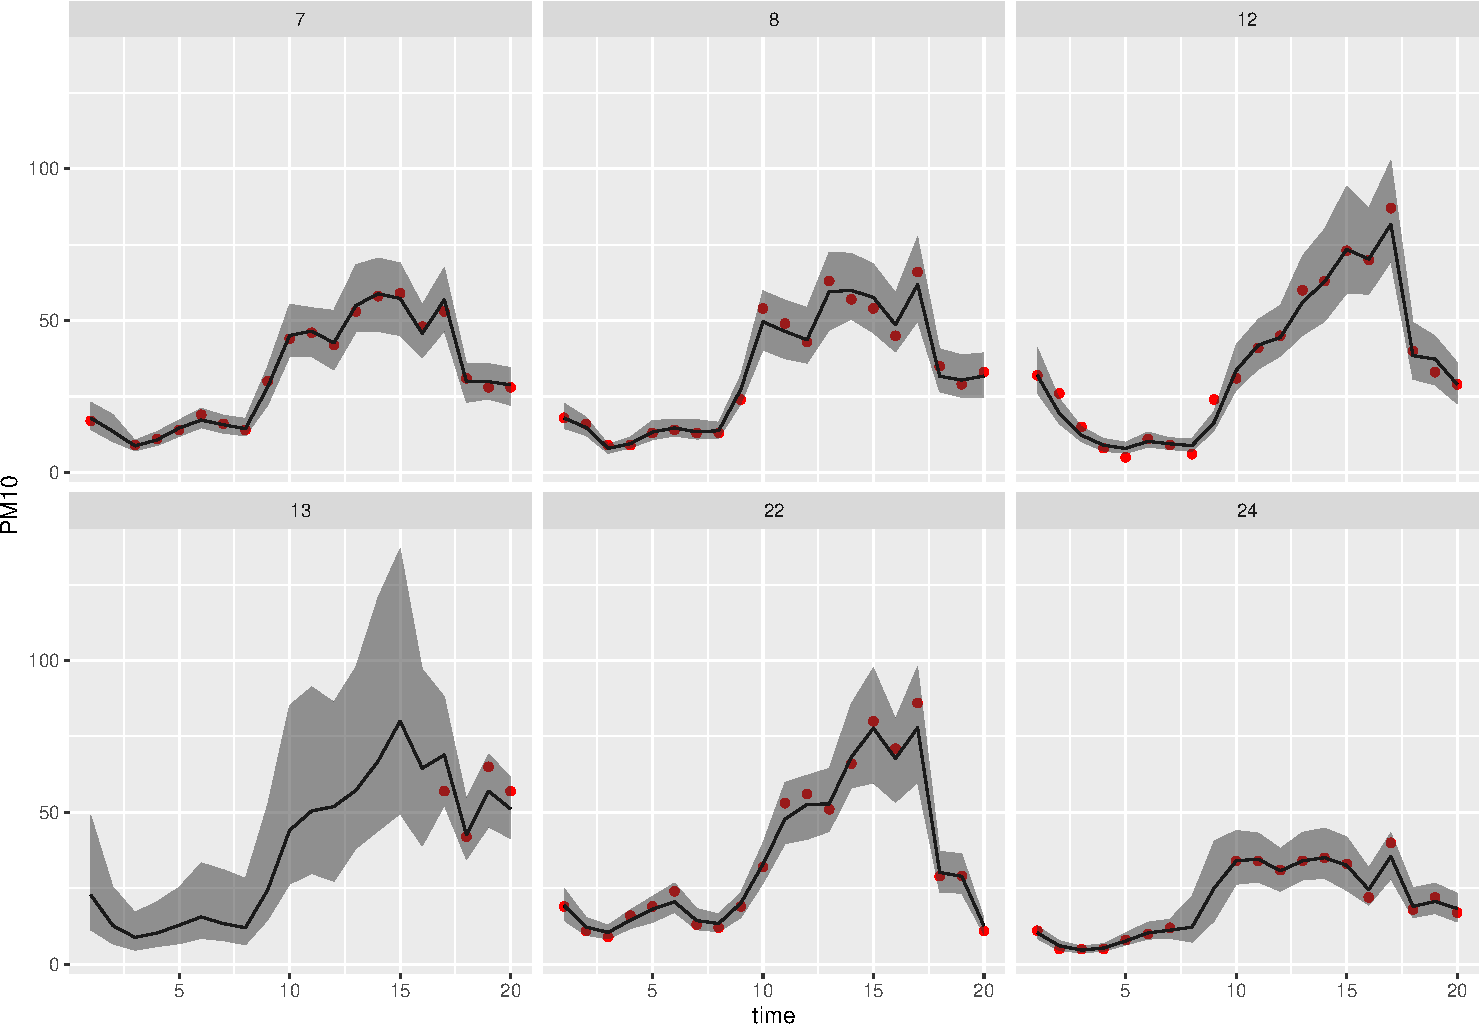
\includegraphics[width=0.7\linewidth]{Part3_Spatial_files/figure-beamer/unnamed-chunk-32-1} \end{center}
\end{frame}

\begin{frame}{Prediction is space}
\protect\hypertarget{prediction-is-space}{}
\begin{itemize}
\item
  To do this we need to have the covariates over the space of interest.
\item
  The should cover the whole mesh
\end{itemize}
\end{frame}

\begin{frame}[fragile]{Expanding the covariates: the
\texttt{bru\_fill\_missing}}
\protect\hypertarget{expanding-the-covariates-the-bru_fill_missing}{}
\tiny

\begin{Shaded}
\begin{Highlighting}[]
\CommentTok{\# read the covariate values}
\NormalTok{alt }\OtherTok{=} \FunctionTok{read.table}\NormalTok{(}\StringTok{"Data/Piemonte\_data/Altitude.dat"}\NormalTok{)}
\DocumentationTok{\#\# object with altitude, this does not cover the whole mesh!}
\NormalTok{dem }\OtherTok{=} \FunctionTok{SpatialPixelsDataFrame}\NormalTok{(}\AttributeTok{points =} \FunctionTok{cbind}\NormalTok{(alt[,}\DecValTok{1}\NormalTok{],}
\NormalTok{                                            alt[,}\DecValTok{2}\NormalTok{]),}
                             \AttributeTok{data =} \FunctionTok{data.frame}\NormalTok{(}\AttributeTok{dem =}\NormalTok{ alt[,}\DecValTok{3}\NormalTok{]))}
\DocumentationTok{\#\# create another object which  does cover the whole mesh}
\NormalTok{large\_grid }\OtherTok{=} \FunctionTok{expand\_grid}\NormalTok{(}\AttributeTok{x =} \FunctionTok{seq}\NormalTok{(}\DecValTok{250}\NormalTok{, }\DecValTok{580}\NormalTok{,}\DecValTok{4}\NormalTok{),}
                         \AttributeTok{y =} \FunctionTok{seq}\NormalTok{(}\DecValTok{4810}\NormalTok{, }\DecValTok{5210}\NormalTok{,}\DecValTok{4}\NormalTok{))}
\CommentTok{\# expand dem {-}{-}{-}{-}{-}{-}{-}{-}{-}{-}{-}{-}{-}{-}{-}{-}{-}{-}{-}{-}{-}{-}{-}{-}{-}{-}{-}{-}{-}{-}{-}{-}{-}{-}{-}{-}{-}{-}{-}{-}{-}{-}{-}{-}{-}{-}{-}{-}{-}{-}{-}{-}{-}{-}{-}{-}{-}{-}{-}{-}{-}{-}}
\NormalTok{dem\_large }\OtherTok{=} \FunctionTok{SpatialPixelsDataFrame}\NormalTok{(}\AttributeTok{points =}\NormalTok{ large\_grid,}
                                   \AttributeTok{data =} \FunctionTok{data.frame}\NormalTok{(}\AttributeTok{dem =} 
                                                       \FunctionTok{rep}\NormalTok{(}\ConstantTok{NA}\NormalTok{,}\FunctionTok{length}\NormalTok{(large\_grid}\SpecialCharTok{$}\NormalTok{x))))}

\CommentTok{\# Use bru\_fill\_missing to fill the new object}
\NormalTok{dem\_large}\SpecialCharTok{$}\NormalTok{dem }\OtherTok{\textless{}{-}} \FunctionTok{bru\_fill\_missing}\NormalTok{(}\AttributeTok{data =}\NormalTok{ dem,}
                       \AttributeTok{where =}\NormalTok{ dem\_large,}
                       \AttributeTok{values =}\NormalTok{ dem\_large}\SpecialCharTok{$}\NormalTok{dem)}
\end{Highlighting}
\end{Shaded}

\normalsize
\end{frame}

\begin{frame}{Expanding the covariates: the \texttt{bru\_fill\_missing}}
\protect\hypertarget{expanding-the-covariates-the-bru_fill_missing-1}{}
\begin{center}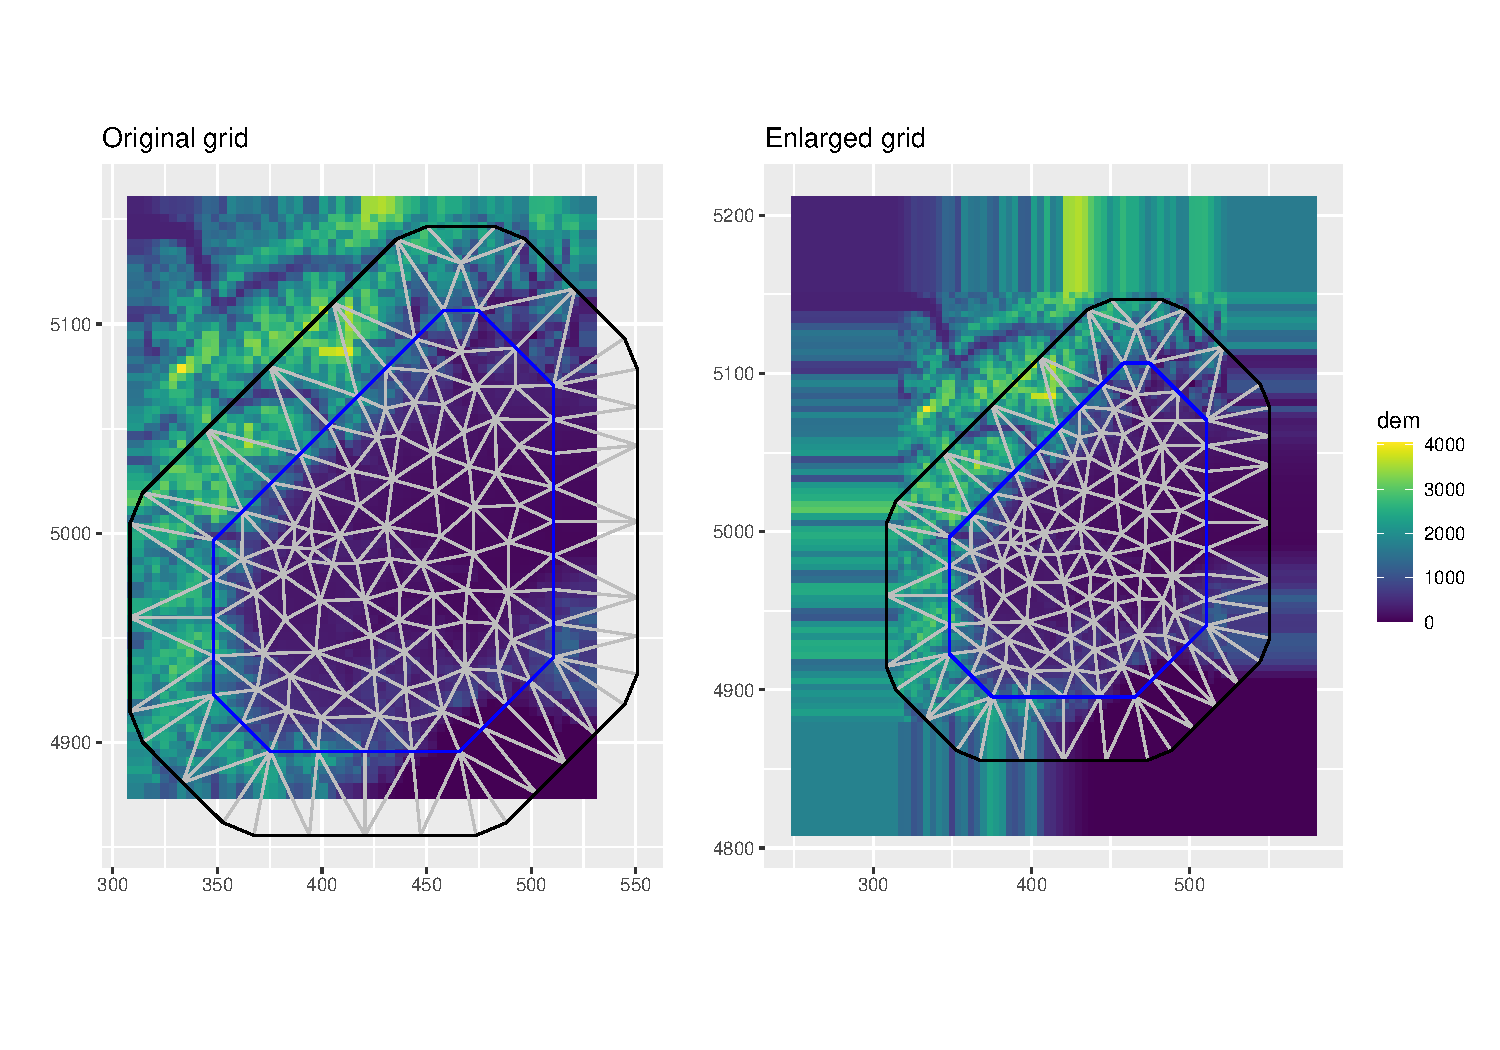
\includegraphics[width=0.7\linewidth]{Part3_Spatial_files/figure-beamer/unnamed-chunk-34-1} \end{center}

Note: You can do this with your favourite method!
\end{frame}

\hypertarget{prediction-in-space}{%
\section{Prediction in space}\label{prediction-in-space}}

\begin{frame}[fragile]{Prediction in space}
\tiny

\begin{Shaded}
\begin{Highlighting}[]
\CommentTok{\# Create a space time grid }
\NormalTok{pxl }\OtherTok{=} \FunctionTok{pixels}\NormalTok{(mesh, }\AttributeTok{nx =} \DecValTok{200}\NormalTok{, }\AttributeTok{ny =} \DecValTok{200}\NormalTok{, }\AttributeTok{mask =}\NormalTok{ shape)}
\NormalTok{ips2 }\OtherTok{\textless{}{-}} \FunctionTok{ipoints}\NormalTok{(}\AttributeTok{domain =} \FunctionTok{c}\NormalTok{(}\DecValTok{1}\SpecialCharTok{:}\DecValTok{5}\NormalTok{), }\AttributeTok{name =} \StringTok{"time"}\NormalTok{)}
\NormalTok{pxl\_time }\OtherTok{\textless{}{-}} \FunctionTok{cbind}\NormalTok{(}\FunctionTok{cprod}\NormalTok{(pxl,ips2), }\FunctionTok{data.frame}\NormalTok{(}\AttributeTok{temp =} \DecValTok{0}\NormalTok{))}

\NormalTok{pred\_space }\OtherTok{=} \FunctionTok{predict}\NormalTok{(fit, pxl\_time, }
                      \SpecialCharTok{\textasciitilde{}}\NormalTok{ Intercept }\SpecialCharTok{+}\NormalTok{ SPDE }\SpecialCharTok{+}
                       \FunctionTok{dem\_eval}\NormalTok{(inlabru}\SpecialCharTok{:::}\FunctionTok{eval\_SpatialDF}\NormalTok{(dem\_large,}
\NormalTok{                                                         .data.)) }\SpecialCharTok{+}
                       \FunctionTok{temp\_eval}\NormalTok{(inlabru}\SpecialCharTok{:::}\FunctionTok{eval\_SpatialDF}\NormalTok{(temp\_large,}
\NormalTok{                                                          .data.,}
                                                          \AttributeTok{selector =} \StringTok{"time"}\NormalTok{)))}
\end{Highlighting}
\end{Shaded}

\normalsize
\end{frame}

\begin{frame}{Prediction in space}
\protect\hypertarget{prediction-in-space-1}{}
\begin{center}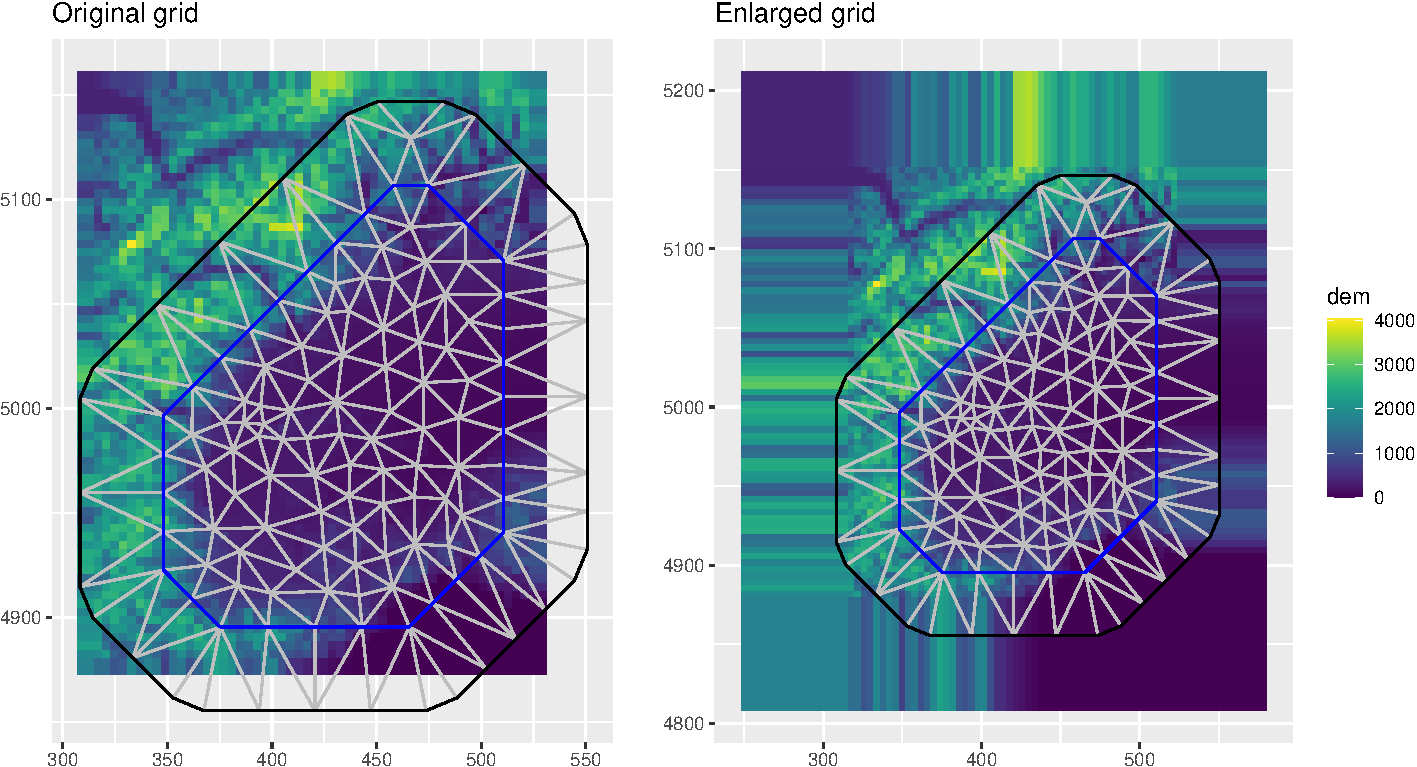
\includegraphics[width=0.9\linewidth]{Part3_Spatial_files/figure-beamer/unnamed-chunk-37-1} \end{center}
\end{frame}

\begin{frame}[fragile]{Samples form the fitted model}
\protect\hypertarget{samples-form-the-fitted-model}{}
It is also possible to generate from the fitted model \tiny

\begin{Shaded}
\begin{Highlighting}[]
\NormalTok{sim\_space }\OtherTok{=} \FunctionTok{generate}\NormalTok{(fit, pxl\_time, }
                      \SpecialCharTok{\textasciitilde{}} \FunctionTok{exp}\NormalTok{(Intercept }\SpecialCharTok{+}\NormalTok{ SPDE }\SpecialCharTok{+}
                       \FunctionTok{dem\_eval}\NormalTok{(inlabru}\SpecialCharTok{:::}\FunctionTok{eval\_SpatialDF}\NormalTok{(dem\_large,}
\NormalTok{                                                         .data.)) }\SpecialCharTok{+}
                       \FunctionTok{temp\_eval}\NormalTok{(inlabru}\SpecialCharTok{:::}\FunctionTok{eval\_SpatialDF}\NormalTok{(temp\_large,}
\NormalTok{                                                          .data.,}
                                                          \AttributeTok{selector =} \StringTok{"time"}\NormalTok{))),}
                     \AttributeTok{n.samples =} \DecValTok{2}\NormalTok{)}
\end{Highlighting}
\end{Shaded}

\normalsize

This can be usefull as the posterior means are always smoother than the
``real'' field
\end{frame}

\begin{frame}{Samples form the fitted model}
\protect\hypertarget{samples-form-the-fitted-model-1}{}
\begin{center}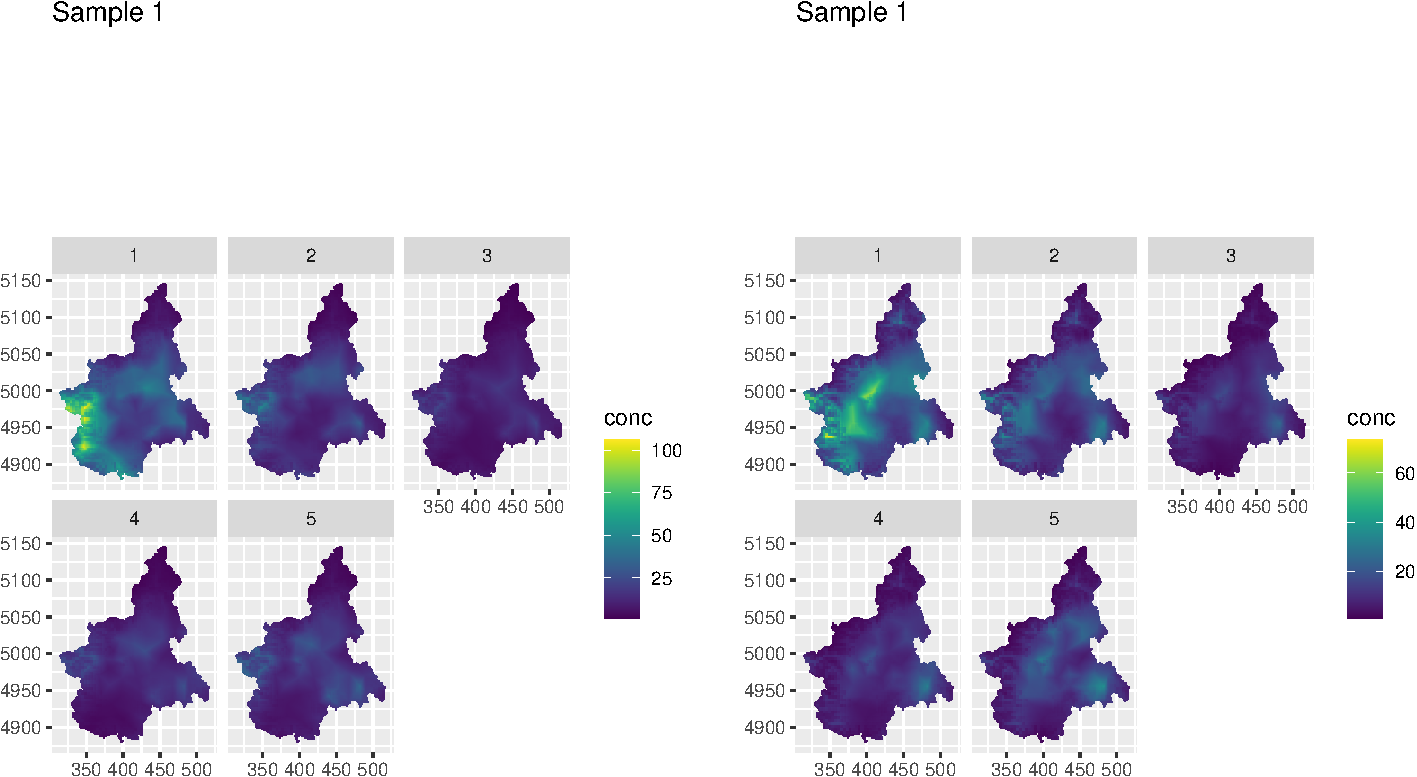
\includegraphics[width=0.9\linewidth]{Part3_Spatial_files/figure-beamer/unnamed-chunk-39-1} \end{center}
\end{frame}

\begin{frame}[fragile]{Some concluding remark}
\protect\hypertarget{some-concluding-remark}{}
\begin{itemize}
\item
  The functions \texttt{predict()} and \texttt{generate()} in
  \texttt{inlabru} use the \texttt{INLA} function
  \texttt{inla.posterior.sample()} internally.
\item
  \texttt{inlabru} is a wrapper around \texttt{INLA} so all the internal
  computations are identical!
\item
  \texttt{inlabru} makes handling of spatial object a lot easier
\item
  Transition from \texttt{sp} to \texttt{sf}/\texttt{terra} some
  changing can be expected
\end{itemize}
\end{frame}

\begin{frame}{}
\protect\hypertarget{section-1}{}
\Large

Thank you for your attention!

\normalsize

If you have any doubts or questions, please write :
\url{sara.martino@math.ntnu.no}

\begin{center}
\includegraphics[width=0.3\linewidth]{graphics/smiley_small} \end{center}
\end{frame}

\end{document}
